%!TEX TS-program = xelatex
\documentclass[11pt]{article}

\usepackage[english]{babel}

\usepackage{amsmath,amssymb,amsfonts}
\usepackage[utf8]{inputenc}
\usepackage[T1]{fontenc}
\usepackage{stix}
\usepackage[scaled]{helvet}
\usepackage[scaled]{inconsolata}

\usepackage{lastpage}

\usepackage{setspace}

\usepackage{ccicons}

\usepackage[hang,flushmargin]{footmisc}

\usepackage{geometry}

\setlength{\parindent}{0pt}
\setlength{\parskip}{6pt plus 2pt minus 1pt}

\usepackage{fancyhdr}
\renewcommand{\headrulewidth}{0pt}

\usepackage{subfig}\providecommand{\tightlist}{%
  \setlength{\itemsep}{0pt}\setlength{\parskip}{0pt}}

\makeatletter
\newcounter{tableno}
\newenvironment{tablenos:no-prefix-table-caption}{
  \caption@ifcompatibility{}{
    \let\oldthetable\thetable
    \let\oldtheHtable\theHtable
    \renewcommand{\thetable}{tableno:\thetableno}
    \renewcommand{\theHtable}{tableno:\thetableno}
    \stepcounter{tableno}
    \captionsetup{labelformat=empty}
  }
}{
  \caption@ifcompatibility{}{
    \captionsetup{labelformat=default}
    \let\thetable\oldthetable
    \let\theHtable\oldtheHtable
    \addtocounter{table}{-1}
  }
}
\makeatother

\usepackage{array}
\newcommand{\PreserveBackslash}[1]{\let\temp=\\#1\let\\=\temp}
\let\PBS=\PreserveBackslash

\usepackage[breaklinks=true]{hyperref}
\hypersetup{colorlinks,%
citecolor=blue,%
filecolor=blue,%
linkcolor=blue,%
urlcolor=blue}
\usepackage{url}

\usepackage{caption}
\setcounter{secnumdepth}{0}
\usepackage{cleveref}

\usepackage{graphicx}
\makeatletter
\def\maxwidth{\ifdim\Gin@nat@width>\linewidth\linewidth
\else\Gin@nat@width\fi}
\makeatother
\let\Oldincludegraphics\includegraphics
\renewcommand{\includegraphics}[1]{\Oldincludegraphics[width=\maxwidth]{#1}}

\usepackage{longtable}
\usepackage{booktabs}

\usepackage{color}
\usepackage{fancyvrb}
\newcommand{\VerbBar}{|}
\newcommand{\VERB}{\Verb[commandchars=\\\{\}]}
\DefineVerbatimEnvironment{Highlighting}{Verbatim}{commandchars=\\\{\}}
% Add ',fontsize=\small' for more characters per line
\usepackage{framed}
\definecolor{shadecolor}{RGB}{248,248,248}
\newenvironment{Shaded}{\begin{snugshade}}{\end{snugshade}}
\newcommand{\KeywordTok}[1]{\textcolor[rgb]{0.13,0.29,0.53}{\textbf{#1}}}
\newcommand{\DataTypeTok}[1]{\textcolor[rgb]{0.13,0.29,0.53}{#1}}
\newcommand{\DecValTok}[1]{\textcolor[rgb]{0.00,0.00,0.81}{#1}}
\newcommand{\BaseNTok}[1]{\textcolor[rgb]{0.00,0.00,0.81}{#1}}
\newcommand{\FloatTok}[1]{\textcolor[rgb]{0.00,0.00,0.81}{#1}}
\newcommand{\ConstantTok}[1]{\textcolor[rgb]{0.00,0.00,0.00}{#1}}
\newcommand{\CharTok}[1]{\textcolor[rgb]{0.31,0.60,0.02}{#1}}
\newcommand{\SpecialCharTok}[1]{\textcolor[rgb]{0.00,0.00,0.00}{#1}}
\newcommand{\StringTok}[1]{\textcolor[rgb]{0.31,0.60,0.02}{#1}}
\newcommand{\VerbatimStringTok}[1]{\textcolor[rgb]{0.31,0.60,0.02}{#1}}
\newcommand{\SpecialStringTok}[1]{\textcolor[rgb]{0.31,0.60,0.02}{#1}}
\newcommand{\ImportTok}[1]{#1}
\newcommand{\CommentTok}[1]{\textcolor[rgb]{0.56,0.35,0.01}{\textit{#1}}}
\newcommand{\DocumentationTok}[1]{\textcolor[rgb]{0.56,0.35,0.01}{\textbf{\textit{#1}}}}
\newcommand{\AnnotationTok}[1]{\textcolor[rgb]{0.56,0.35,0.01}{\textbf{\textit{#1}}}}
\newcommand{\CommentVarTok}[1]{\textcolor[rgb]{0.56,0.35,0.01}{\textbf{\textit{#1}}}}
\newcommand{\OtherTok}[1]{\textcolor[rgb]{0.56,0.35,0.01}{#1}}
\newcommand{\FunctionTok}[1]{\textcolor[rgb]{0.00,0.00,0.00}{#1}}
\newcommand{\VariableTok}[1]{\textcolor[rgb]{0.00,0.00,0.00}{#1}}
\newcommand{\ControlFlowTok}[1]{\textcolor[rgb]{0.13,0.29,0.53}{\textbf{#1}}}
\newcommand{\OperatorTok}[1]{\textcolor[rgb]{0.81,0.36,0.00}{\textbf{#1}}}
\newcommand{\BuiltInTok}[1]{#1}
\newcommand{\ExtensionTok}[1]{#1}
\newcommand{\PreprocessorTok}[1]{\textcolor[rgb]{0.56,0.35,0.01}{\textit{#1}}}
\newcommand{\AttributeTok}[1]{\textcolor[rgb]{0.77,0.63,0.00}{#1}}
\newcommand{\RegionMarkerTok}[1]{#1}
\newcommand{\InformationTok}[1]{\textcolor[rgb]{0.56,0.35,0.01}{\textbf{\textit{#1}}}}
\newcommand{\WarningTok}[1]{\textcolor[rgb]{0.56,0.35,0.01}{\textbf{\textit{#1}}}}
\newcommand{\AlertTok}[1]{\textcolor[rgb]{0.94,0.16,0.16}{#1}}
\newcommand{\ErrorTok}[1]{\textcolor[rgb]{0.64,0.00,0.00}{\textbf{#1}}}
\newcommand{\NormalTok}[1]{#1}

\newlength{\cslhangindent}
\setlength{\cslhangindent}{1.5em}
\newlength{\csllabelwidth}
\setlength{\csllabelwidth}{3em}
\newenvironment{CSLReferences}[3] % #1 hanging-ident, #2 entry spacing
 {% don't indent paragraphs
  \setlength{\parindent}{0pt}
  % turn on hanging indent if param 1 is 1
  \ifodd #1 \everypar{\setlength{\hangindent}{\cslhangindent}}\ignorespaces\fi
  % set entry spacing
  \ifnum #2 > 0
  \setlength{\parskip}{#2\baselineskip}
  \fi
 }%
 {}
\usepackage{calc} % for \widthof, \maxof
\newcommand{\CSLBlock}[1]{#1\hfill\break}
\newcommand{\CSLLeftMargin}[1]{\parbox[t]{\maxof{\widthof{#1}}{\csllabelwidth}}{#1}}
\newcommand{\CSLRightInline}[1]{\parbox[t]{\linewidth}{#1}}
\newcommand{\CSLIndent}[1]{\hspace{\cslhangindent}#1}\geometry{verbose,letterpaper,tmargin=2.5cm,bmargin=2.5cm,lmargin=2.5cm,rmargin=4.5cm}

\usepackage{lineno}
\usepackage[nolists,noheads]{endfloat}

\pagestyle{plain}

\doublespacing

\fancypagestyle{normal}
{
  \fancyhf{}
  \fancyfoot[R]{\footnotesize\sffamily\thepage\ of \pageref*{LastPage}}
}
\begin{document}
\thispagestyle{empty}
{\Large\bfseries\sffamily Evaluating ecological uniqueness over broad
spatial extents using species distribution modelling}
\vskip 5em

Gabriel\,Dansereau\,\textsuperscript{1,2,*}\quad Pierre\,Legendre\,\textsuperscript{1,2}\quad Timothée\,Poisot\,\textsuperscript{1,2}

\textsuperscript{1}\,Département de sciences biologiques, Université de
Montréal, Montréal, Canada\quad \textsuperscript{2}\,Québec Centre for
Biodiversity Science, Montréal, Canada

\textsuperscript{*}\,\,\texttt{gabriel.dansereau@umontreal.ca}

\vfill
This work is released by its authors under a CC-BY 4.0 license\hfill\ccby\\
Last revision: \emph{\today}

\clearpage
\thispagestyle{empty}

\vfill
\textbf{\sffamily Abstract: }Local contributions to beta diversity
(LCBD) can be used to identify sites with high ecological uniqueness and
exceptional species composition within a region of interest. Yet, these
indices are typically used on local or regional scales with relatively
few sites, as they require information on complete community
compositions difficult to acquire on larger scales. Here, we
investigated how LCBD indices can be predicted over broad spatial
extents using species distribution modelling and examined the effect of
scale changes on beta diversity quantification. We used Bayesian
additive regression trees (BARTs) to predict warbler species
distributions in North America based on observations recorded in the
eBird database. We then calculated LCBD indices for observed and
predicted data and compared the site-wise difference using direct
comparison, a spatial association test, and generalized linear
regression. We also examined the relationship between LCBD values and
species richness in different regions and at various spatial extents.
Our results showed that species distribution models provided uniqueness
estimates highly correlated with observed data. The form and variance of
the LCBD-richness relationship varied according to the region and the
total extent size. The relationship was also affected by the proportion
of rare species in the communities. Therefore, sites identified as
unique over broad spatial extents may vary according to regional
characteristics. These results show that species distribution modelling
can be used to predict ecological uniqueness over broad spatial extents,
which could help identify beta diversity hotspots and important targets
for conservation purposes in unsampled locations.
\vfill

\clearpage
\linenumbers
\pagestyle{normal}

\hypertarget{introduction}{%
\section{Introduction}\label{introduction}}

Beta diversity, defined as the variation in species composition among
sites in a geographic region of interest (Legendre, Borcard, and
Peres-Neto 2005), is an essential measure to describe the organization
of biodiversity through space. Total beta diversity within a community
can be partitioned into local contributions to beta diversity (LCBD)
(Legendre and De Cáceres 2013), which allow the identification of sites
with exceptional species composition, hence unique biodiversity and
potential conservation value. Sites with unique community composition
often differ from those with high species richness, possibly as they
harbour rare species or help maintain beta diversity (da Silva,
Hernández, and Heino 2018; Heino et al. 2017; Landeiro et al. 2018).
Hence, focusing on uniqueness can prove helpful as a complementary
approach to species richness (Heino and Grönroos 2017; da Silva,
Hernández, and Heino 2018; Yao et al. 2021; Dubois, Proulx, and Pellerin
2020). However, the use of LCBD indices is currently limited in two
ways. First, LBCD indices are typically used on data collected over
local or regional scales with relatively few sites, for example, on fish
communities at intervals along a river or stream (Legendre and De
Cáceres 2013). Second, LCBD calculation methods require complete
information on community composition; thus, they are inappropriate for
partially sampled sites (e.g., where data for some species are missing
or uncertain) and cannot directly provide assessments for unsampled
ones. Accordingly, this method is of limited use to identify areas with
exceptional biodiversity in regions with sparse sampling. However,
predictive approaches offer an opportunity to overcome such limitations,
as computational methods often uncover novel ecological insights from
existing data (Poisot et al. 2019), including in lesser-known locations
and on larger spatial scales.

Species distribution models (SDMs) (Guisan and Thuiller 2005) can bring
a new perspective to LCBD studies by filling in gaps in community
composition data to perform analyses on broader scales. Single-species
SDMs aim at predicting the distribution of a species in unsampled
locations based on information (such as environmental data) from sampled
locations with reported occurrences. Many approaches allow going from
single-species SDMs to a whole community on which to evaluate
community-level metrics, yet their relevance has not been explicitly
evaluated for ecological uniqueness and LCBD indices. The most
straightforward approach is stacked distribution models (S-SDMs)
(Ferrier and Guisan 2006; Guisan and Rahbek 2011). Single-species SDMs
are first performed separately, then combined to form a community
prediction on which community-level analyses can be applied. S-SDMs tend
to overestimate species richness (Dubuis et al. 2011; D'Amen et al.
2015; Zurell et al. 2020), which could result from thresholding the
probabilities into presence-absence data before stacking the species
distributions (Calabrese et al. 2014). Summing the occurrence
probabilities without applying a threshold is an alternative (Calabrese
et al. 2014), but it may limit some analyses as it does not return
species identities for every site (Zurell et al. 2020), as is required
with LCBD calculations. In comparison, joint species distribution models
(JSDMs)(Pollock et al. 2014) try to improve predictions by incorporating
species co-occurrence or shared environmental responses into the models.
However, these models do not always improve community-level predictions
compared to S-SDMs (Zurell et al. 2020). Spatially explicit species
assemblage modelling (SESAM) (Guisan and Rahbek 2011), hierarchical
modelling of species communities (HMSC) (Ovaskainen et al. 2017), and
Bayesian networks (BN) (Staniczenko et al. 2017) are other alternatives
that could yield better community predictions than S-SDMs. On the other
hand, they add methodological and computational overload, impeding their
use for broad spatial extents. Moreover, their relevance for community
prediction is often validated against extensive work on species
richness. By comparison, ecological uniqueness and LCBD indices have
rarely been used in predictive frameworks. Therefore, S-SDMs may prove
an appropriate first step to establish some prediction baselines.

Combining LCBD indices with a predictive approach through SDMs will
allow measuring uniqueness over broader spatial extents, across
continuous landscapes, and on a higher number of sites than what has
previously been studied. LCBD scores have typically been used at local
or regional scales with relatively few sites (up to 60 sites on extents
covering 10 km to 400 km, Legendre and De Cáceres 2013; da Silva and
Hernández 2014; Heino et al. 2017; Heino and Grönroos 2017). Some
studies did use the measure over broader, near-continental extents (Yang
et al. 2015; Poisot et al. 2017; Taranu, Pinel-Alloul, and Legendre
2020), but the total number of sites in these studies were relatively
small (maximum 51 sites). Recent studies also investigated LCBD and beta
diversity on sites distributed in contiguous grids or as pixels, hence
uniform sampling intervals and no spatial gaps, but these did not cover
large extents and a high number of sites (up to 1250 sites and 6
km\textsuperscript{2}, Tan et al. 2017, 2019; Legendre and Condit 2019;
D'Antraccoli et al. 2020). Two recent studies have, however, adopted
promising predictive approaches on regional extents. First, Niskanen et
al. (2017) predicted LCBD values of plant communities (and three other
diversity measures) on a continuous scale and a high number of sites
(\textgreater{} 25,000) using Boosted Regression Trees (BRTs). However,
they modelled the diversity measures directly after calculating them on
a smaller number of sampled sites. Second, Vasconcelos, Nascimento, and
Prado (2018) used ecological niche models (ENMs) to predict anurans
ecological niches according to actual and forecasted environmental
conditions, then calculated the LCBD values on the predictions to
identify biodiversity hotspots. Using this approach, predicted LCBD
values are calculated in a way closer to the original formulation. This
development of predictive techniques is exciting, especially as it could
be pushed a step further to continental extents, a higher number of
sites, and more species occurrences using SDMs and massive data sources.
Still, it should be accompanied by an investigation of the determinant
of ecological uniqueness in such conditions.

Measuring ecological uniqueness from LCBD indices over broad spatial
extents and spatially continuous data also raises the question of which
sites will be identified as exceptional and for what reason. The method
intends that sites stand out and receive a high LCBD score whenever they
display an exceptional community composition, be it a unique assemblage
of species with high conservation value or a community richer or poorer
than others in the region (Legendre and De Cáceres 2013). Both the
original study and many of the later empirical ones have shown a
negative relationship between LCBD scores and species richness (Legendre
and De Cáceres 2013; da Silva and Hernández 2014; Heino et al. 2017;
Heino and Grönroos 2017), although other studies observed both negative
and positive relationships at different sites (Kong et al. 2017) or
quadrats (Yao et al. 2021). Some studies showed that the direction of
the relationship is related to the percentage of rare species in the
community (da Silva, Hernández, and Heino 2018; Yao et al. 2021).
However, beta diversity and species rarity are both concepts that depend
on scale. For instance, total beta diversity increases with spatial
extent (Barton et al. 2013) and varies because of higher environmental
heterogeneity and sampling of different local species pools (Heino et
al. 2015). Therefore, the LCBD-richness relationship and the effect of
rare species on LCBD values should be investigated over broad spatial
extents, as they might not be constant across scales.

Here, we examined whether species distribution models (SDMs) can be
combined with local contributions to beta diversity (LCBD) to assess
ecological uniqueness over broader spatial extents. We also investigated
the effect of scale changes on beta diversity quantification. We first
predicted species distributions on continental scales using extended
occurrence data from eBird and Bayesian additive regression trees
(BARTs). We then quantified uniqueness with the LCBD measure for both
predicted and observed data. Next, we examined the site-wise difference
using direct comparison, a spatial autocorrelation test, and generalized
linear regression. We then investigated the relationship between
uniqueness and species richness for different regions and scales and
according to the proportion of rare species.

\hypertarget{methods}{%
\section{Methods}\label{methods}}

\hypertarget{occurrence-data}{%
\subsection{Occurrence data}\label{occurrence-data}}

We used occurrence data from eBird (Sullivan et al. 2009) downloaded
through the eBird Basic Data set from June 2019 (eBird Basic Dataset
2019). We restricted our analyses to the New World warbler family
(\emph{Parulidae}) in North America (Canada, the United States, Mexico).
eBird is a semi-structured citizen science data set, meaning that
observations are reported as checklists of species detected in an
observation run (Johnston et al. 2020). Observers can explicitly specify
that their checklist contains all species they could detect and identify
during a sampling event, in which case it is labelled as a ``complete
checklist.'' Using complete checklists instead of regular ones allows
researchers to infer non-detections in locations where detection efforts
occurred, which offers performance gains in species distribution models
(Johnston et al. 2020). Therefore, we selected the data from the
complete checklists only. Our final data set comprised 62 warbler
species and 22,974,330 observations from 9,103,750 checklists. Warblers
are a diverse group with many species, are popular among birders given
their charismatic aspect, and are widely distributed in various habitats
across North America.

\hypertarget{environmental-data}{%
\subsection{Environmental data}\label{environmental-data}}

Our environmental data consisted of climatic data from WorldClim 2.1
(Fick and Hijmans 2017) and land cover data from the Copernicus Global
Land Service (Buchhorn et al. 2019). We restricted these data to a
spatial extent comprised between -145.0 and -50.0 degrees of longitude
and between 20.0 and 75.0 degrees of latitude. First, the WorldClim data
consist of spatially interpolated monthly climate data for global land
areas. We used the standard \textsc{bioclim} variables (Booth et al.
2014) from WorldClim 2.1, which represent annual trends, ranges, and
extremes of temperature and precipitation, but selected only 8 out of
the 19 ones to avoid redundancy (bio1, bio2, bio5, bio6, bio12, bio13,
bio14, bio15). We downloaded the data at a resolution of 10 arcminutes
(around 18 km\textsuperscript{2} at the equator), the coarsest
resolution available, which should mitigate potential imprecision in the
eBird data regarding the extent of the sampled areas in each observation
checklist. Moreover, some studies have argued that coarser resolutions
lead to less overestimation of species richness and better
identification of bird biodiversity hotspots given the patchiness of
observation data (Hurlbert and Jetz 2007). We acknowledge that using an
arcminutes-based resolution means that the surface area of our pixels
will not be equal depending on the latitude.

Second, the Copernicus data are a set of variables representing ten land
cover classes (e.g., crops, trees, urban areas) and measured as a
percentage of land cover. The data are only available at a finer
resolution of 100 m. We coarsened them to the same ten arcminute
resolution as the WorldClim data by averaging the pixels' cover fraction
values. We removed two variables (moss and snow) from our predictive
models as their cover fraction was 0\% on all sites with warbler
observations.

\hypertarget{species-distribution-models}{%
\subsection{Species distribution
models}\label{species-distribution-models}}

We converted the occurrence data to a presence-absence format compatible
with community analyses. We considered every pixel from our ten
arcminutes environmental layers as a site and then verified, for each
species, if there was a single observation in every site. Finally, we
recorded the outcome as a binary value: present (1) if a species was
ever recorded in a site and absent (0) if it was not. Complete
checklists help ensure that these zeros represent non-detections, rather
than the species not being reported; hence we considered them as absence
data, similar to Johnston et al. (2020), although we recognize that
there exists a doubt on whether these truly represent non-detections.

We predicted species distribution data on continuous scales from our
presence-absence data using Bayesian Additive Regression Trees (BARTs)
(Chipman, George, and McCulloch 2010), a classification and regression
trees method recently suggested for species distribution modelling
(Carlson 2020). BARTs are based on an ensemble of trees, similarly to
Boosted Regression Trees and Random Forest, but follow a sum-of-trees
model and a Bayesian framework. Trees are first constrained as weak
learners by priors regarding structure and nodes, then updated through
an iterative Bayesian backfitting Markov Chain Monte Carlo (MCMC)
algorithm which ultimately generates a posterior distribution of
predicted classification probabilities (Chipman, George, and McCulloch
2010; Carlson 2020). In the context of species distribution modelling,
BARTs showed high performance when compared to other predictive
algorithms (Konowalik and Nosol 2021; Tytar and Baidashnikov 2021). We
first performed BARTs separately for all species and estimated the
probability of occurrence in all the sites of our region of interest
using the posterior median. We then converted the results to a binary
outcome according to the threshold that maximized the True Skill
Statistic (TSS) for each species, as suggested by Carlson (2020).

\hypertarget{quantification-of-ecological-uniqueness}{%
\subsection{Quantification of ecological
uniqueness}\label{quantification-of-ecological-uniqueness}}

We~used the method of Legendre and De Cáceres (2013) to quantify
compositional uniqueness from overall beta diversity for both the
observed and predicted data. First, we assembled the presence-absence
data by site to form two site-by-species community matrices, one from
observed data, called \(Y\) (39,024 sites by 62 species), and one from
predicted data, called \(\hat Y\) (99,382 sites by 62 species). Next, we
measured species richness per site as the number of species present.
Finally, we removed the sites without any species from the predicted
matrix \(\hat Y\), for a new total of 85,526 sites (this was unnecessary
for the observed matrix \(Y\)). We then applied the Hellinger
transformation to both matrices in order to compute beta diversity from
the community composition data (Legendre and De Cáceres 2013). We
measured total beta diversity as the variance of each community matrix
and calculated the local contributions to beta diversity (LCBD), which
quantify how much a specific site (a row in each matrix) contributes to
the overall variance in the community (Legendre and De Cáceres 2013).
High LCBD values indicate a unique community composition, while low
values indicate a more common species set. We note that our LCBD values,
which add up to 1 because the values are divided by the total
sum-of-squares of the data matrix, were very low given the high number
of sites in both \(Y\) and \(\hat Y\). However, the relative difference
between the scores in one set matters more than the absolute value to
differentiate their uniqueness.

\hypertarget{comparison-of-observed-and-predicted-values}{%
\subsection{Comparison of observed and predicted
values}\label{comparison-of-observed-and-predicted-values}}

We performed three verification to compare the richness and uniqueness
estimates obtained from our predicted distributions to those obtained
with the eBird occurrence data. First, we performed a direct comparison
by subtracting the richness and LCBD estimates obtained from \(Y\) (the
observed data) from the estimates obtained from \(\hat{Y}\) (the
predicted data). To do so, we used the richness estimates as-is but
modified the LCBD values to achieve a non-biased comparison, given that
the values were initially calculated on sets of different lengths.
Therefore, we recomputed the LCBD scores only for the sites for which we
had occurrences in both \(Y\) and \(\hat{Y}\), which mostly corresponded
to the sites in \(Y\), minus a few sites where the SDMs predicted no
species occurrence. We then plotted the richness and LCBD differences to
examine their spatial distributions. Second, we performed the modified
\emph{t} test from Clifford, Richardson, and Hemon (1989) to assess the
correlation between the observed and predicted estimates and test for
spatial association. We performed the test separately for the richness
and the LCBD estimates. Third, we performed Generalized Linear Models
between the observed and predicted estimates and plotted the deviance
residuals to examine their spatial distribution. We used a negative
binomial regression with a log link function for the richness estimates
and a beta regression with a logit link function for the LCBD values,
similar to Heino and Grönroos (2017) and Yao et al. (2021).

\hypertarget{investigation-of-regional-and-scaling-variation}{%
\subsection{Investigation of regional and scaling
variation}\label{investigation-of-regional-and-scaling-variation}}

To investigate possible regional and scaling effects, we recalculated
LCBD values on various subregions at different locations and scales.
First, we selected two subregions of equivalent size (20.0 longitude
degrees by 10.0 latitude degrees) with contrasting richness profiles and
corresponding to different ecoregions to verify if the relationship
between species richness and LCBD values was similar. The first
subregion was in the Northeast (longitude between -80.0 and -60.0,
latitude between 40.0 and 50.0), was mostly species-rich (for both the
observed and predicted data), and corresponded to the Eastern Temperate
Forests level I ecoregion (Commission for Environmental Cooperation
1997). The second subregion was in the Southwest (longitude between
-120.0 and 100.0, latitude between 30.0 and 40.0), was mostly
species-poor, and covered Mediterranean California, North American
Deserts, Temperate Sierras, and Southern Semi-Arid Highlands ecoregions
(Commission for Environmental Cooperation 1997). Second, we recalculated
the LCBD indices at three different extents, starting with a focus on
the Northeast subregion and progressively extending the extent to
encompass the Southwest subregion. We did these two verifications with
both the observed and predicted data but only illustrate the results
with the predicted data as both were qualitatively similar.

\hypertarget{proportion-of-rare-species}{%
\subsection{Proportion of rare
species}\label{proportion-of-rare-species}}

We investigated the effect of the proportion of rare species in the
community on the direction of the relationship between species richness
and LCBD values in our Northeast and Southwest subregions. Following De
Cáceres et al. (2012) and Yao et al. (2021), we classified species as
rare when they occurred in less than 40\% of the sites in each
subregion. We calculated the proportion of rare species for every site.
We then grouped the sites for both subregions depending on whether they
were part of an ascending or a descending portion in the LCBD-richness
relationship. Given that the relationship sometimes displays a
curvilinear form with a positive quadratic term (Heino and Grönroos
2017; Tan et al. 2019), we separated the ascending and descending
portions based on the species richness at the site with the lowest LCBD
value (using the median richness if there were multiple sites). This
value corresponds to the inflection point of the relationships. For
example, the lowest LCBD value was 7.045e-05 in the Northeast subregion
and the corresponding richness was 23. All the sites with more than 23
species were assigned to the ascending portion, and all the sites with
23 species or fewer were assigned to the descending portion. In the
Southwest subregion, the lowest LCBD value and its corresponding
richness were 5.438e-05 and 12, respectively. We then mapped the
ascending and descending groups to view their spatial distribution. We
also examined the distribution of the rare species proportions in both
groups using a kernel density estimation plot. Similar to our previous
verification, we performed this analysis with both observed and
predicted data but once again only illustrate the results with the
predicted data as both were qualitatively similar.

\hypertarget{software}{%
\subsection{Software}\label{software}}

We used \emph{Julia v1.6.1} (Bezanson et al. 2017) for most of the
project and \emph{R v4.1.0} (R Core Team 2021) for some specific steps.
We used the \emph{Julia} package \texttt{SimpleSDMLayers.jl} (Dansereau
and Poisot 2021) as the basic framework for our analyses, to download
the WorldClim 2.1 data, and to map our results through the package's
integration of \texttt{Plots.jl}. We also used \texttt{StatsPlots.jl} to
produce the kernel density estimation plots in our rare species
analysis. We computed the LCBD indices with our own function implemented
in \emph{Julia}, whose results were verified by comparison to the
\texttt{beta.div} function from the package \texttt{adespatial} (Dray et
al. 2021) in \emph{R}. We used the \emph{R} packages \texttt{auk}
(Strimas-Mackey, Miller, and Hochachka 2018) to extract and manipulate
eBird data, \texttt{embarcadero} (Carlson 2020) to perform the BART
models, \texttt{vegan} (Oksanen et al. 2019) to apply the Hellinger
transformations, and \texttt{SpatialPack} (Vallejos, Osorio, and
Bevilacqua 2020) to perform the modified \emph{t} test (with the
function \texttt{modified.ttest}) from Clifford, Richardson, and Hemon
(1989). We used \texttt{MASS} (Venables and Ripley 2002) and
\texttt{betareg} (Cribari-Neto and Zeileis 2010) to perform the negative
binomial and beta regressions, respectively. We also used \texttt{GDAL}
(GDAL/OGR contributors 2021) to coarsen the Copernicus land cover data.
All the scripts required to reproduce the analyses are archived on
Zenodo (\url{https://doi.org/10.5281/zenodo.6024392}).

\hypertarget{results}{%
\section{Results}\label{results}}

\hypertarget{species-distribution-models-generate-relevant-community-predictions}{%
\subsection{Species distribution models generate relevant community
predictions}\label{species-distribution-models-generate-relevant-community-predictions}}

Species richness from observation data (Fig.~\ref{fig:maps}a) was higher
on the East Coast and lower on the West Coast, with many unsampled
patches in the North, South, and Central West. Richness results from SDM
data (Fig.~\ref{fig:maps}b) displayed higher richness on the East Coast
and sites with few or no species up north and in the Central West. There
was no clear latitudinal gradient in richness but rather an East-West
one. Landmarks such as the Rockies and croplands in the Central West
(which should be species-poor habitats) were notably visible on the
maps, separating the East and West. LCBD scores from observation data
(Fig.~\ref{fig:maps}c) were low on the East Coast and higher on the
border of sampled sites in the Central West. They were also higher in
the North and in the South where observations were sparser. Results from
SDM predictions were qualitatively similar (Fig.~\ref{fig:maps}d), with
lower LCBD values in the East and more unique sites in the Central West,
Central Mexico, and some Northern regions. There was no clear
latitudinal gradient, and the East-West contrast, while present, was
less clear than on the richness maps.

\begin{figure}
\hypertarget{fig:maps}{%
\centering
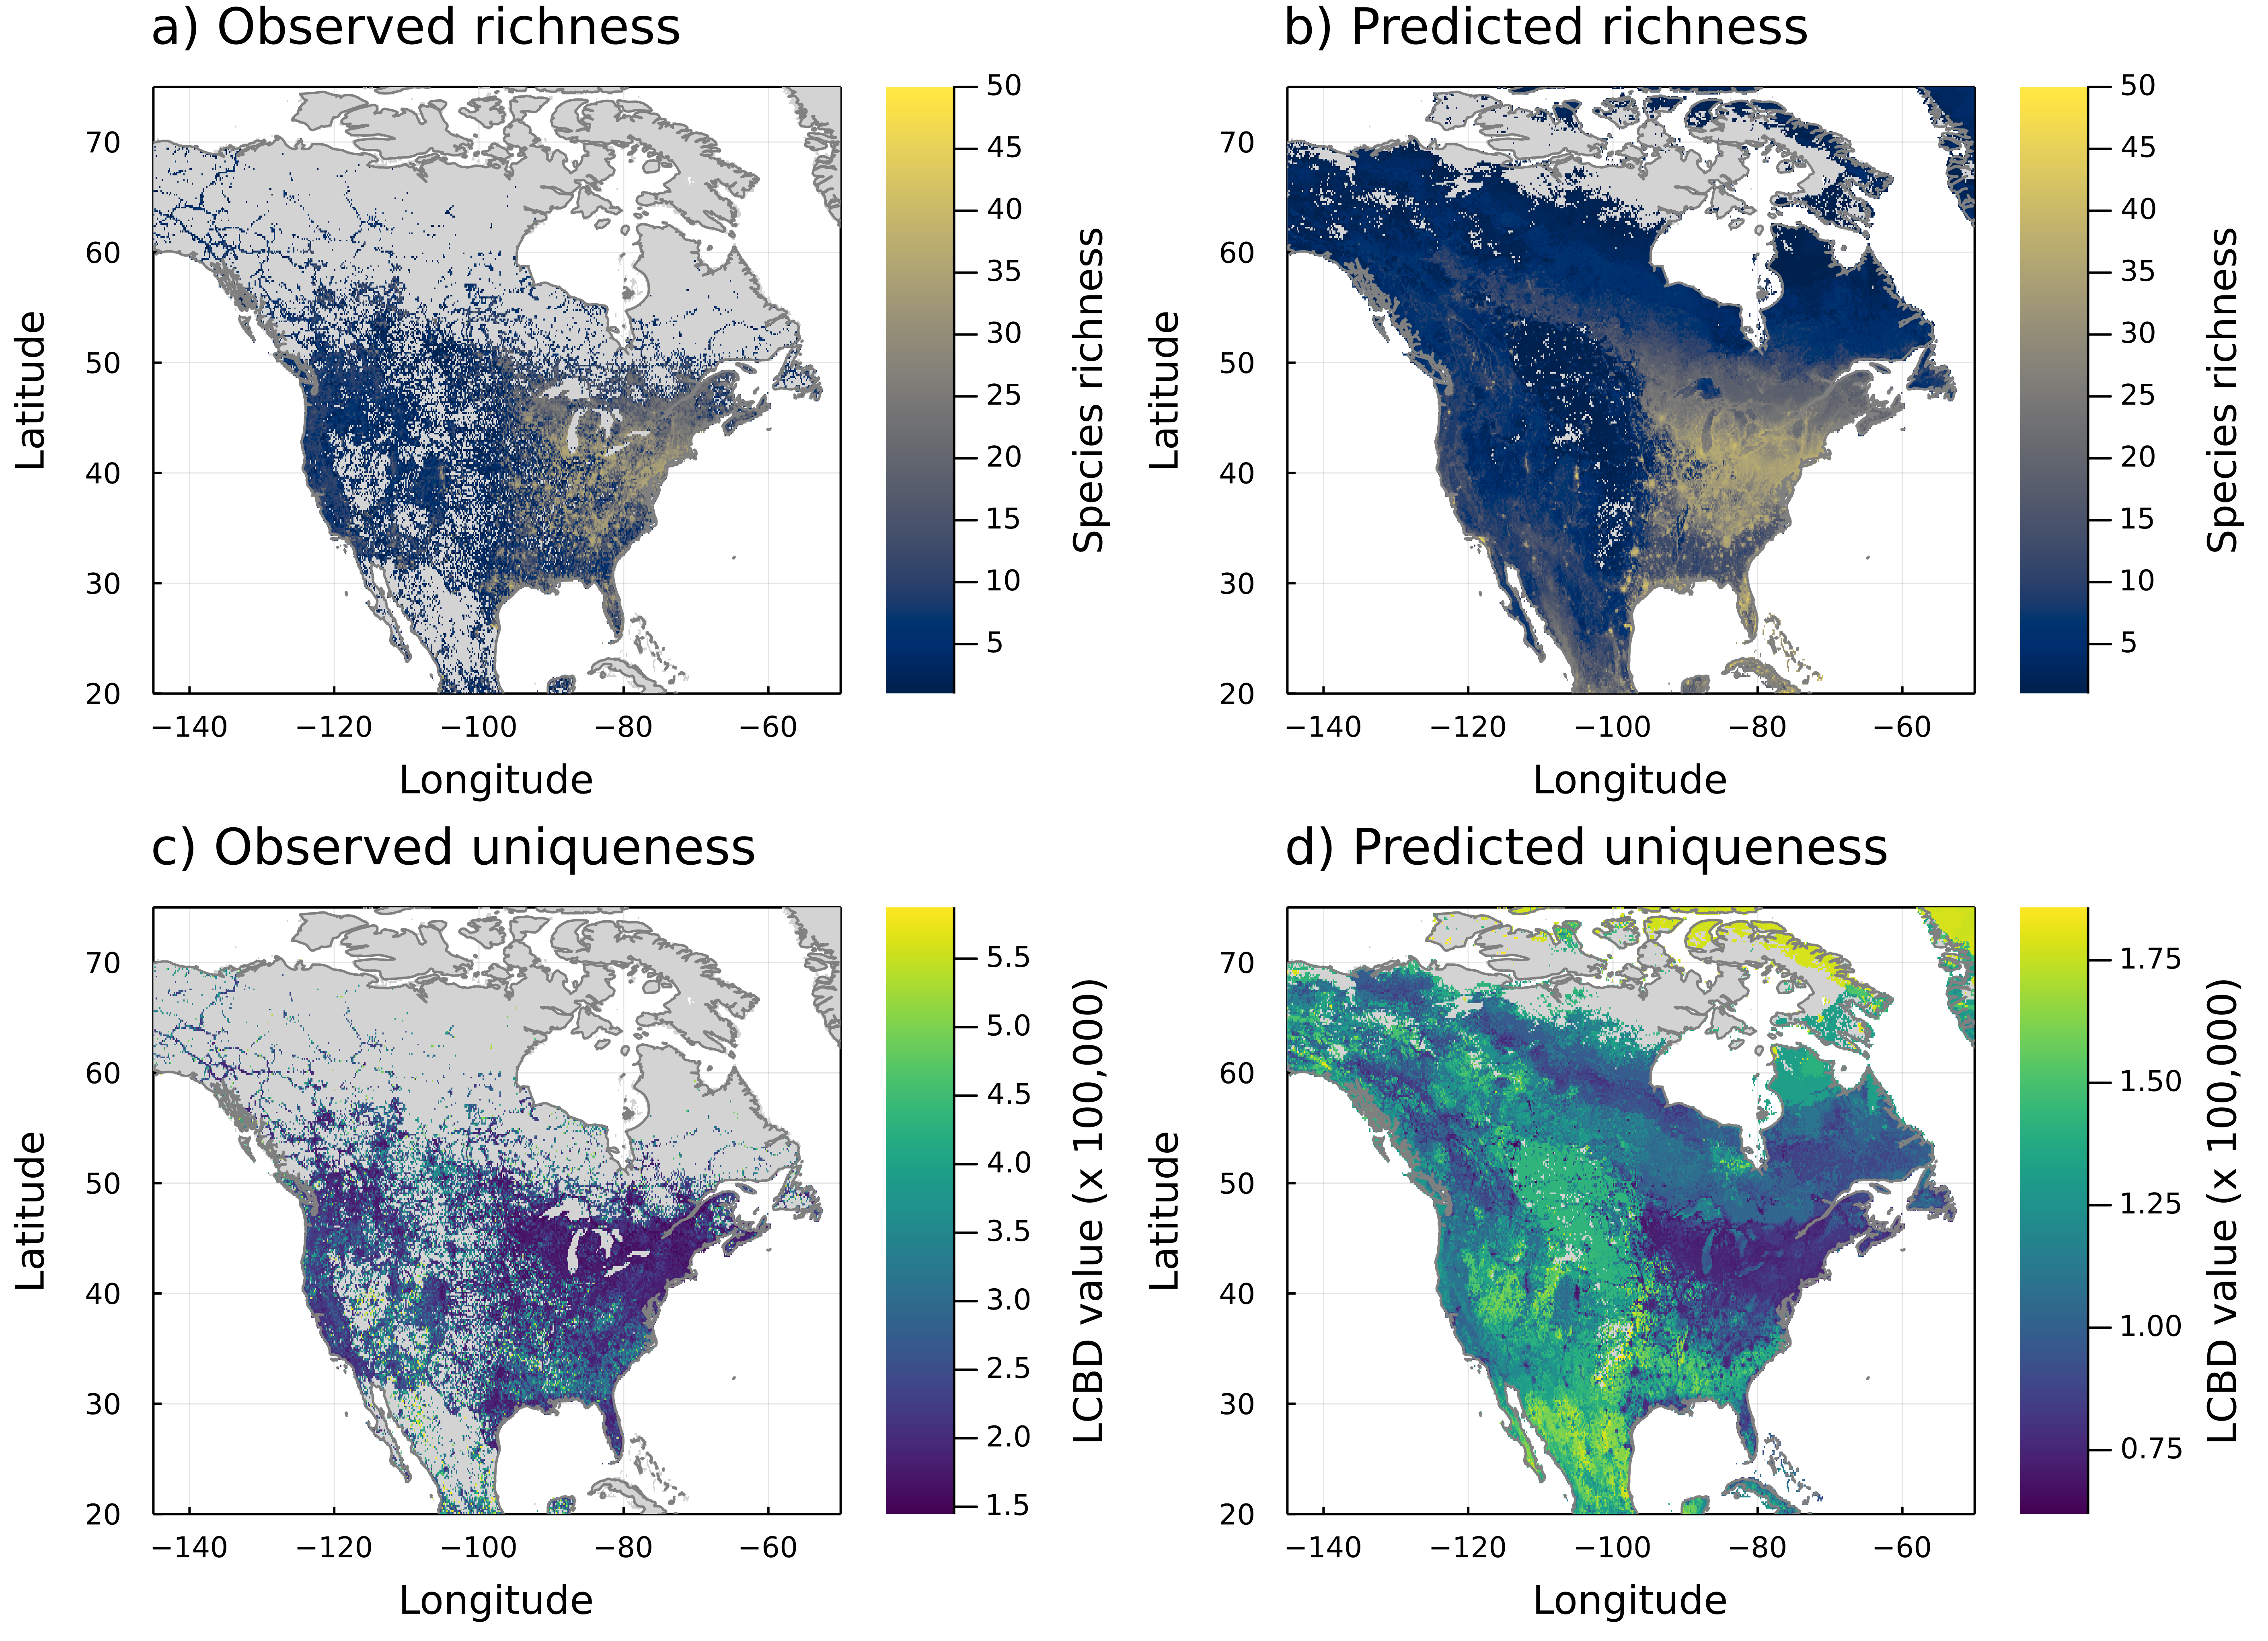
\includegraphics{figures/comparison-combined.png}
\caption{Comparison of species richness and LCBD scores from observed
and predicted warbler occurrences in North America. Values were
calculated for sites representing ten arcminute pixels. We measured
species richness after converting the occurrence data from eBird (a) and
the SDM predictions from our single-species BART models (b) to a
presence-absence format per species. We applied the Hellinger
transformation to the presence-absence data, then calculated the LCBD
values from the variance of the community matrices separately for the
occurrence data (c) and the SDM predictions (d). Areas in light grey
(not on the colour scale) represent mainland sites with environmental
data but without any warbler species present.}\label{fig:maps}
}
\end{figure}

The modified \emph{t} test of Clifford, Richardson, and Hemon (1989)
showed a high correlation between the observed and predicted estimates
of richness and uniqueness, as well as a statistically significant
spatial association between the values. For species richness, the
correlation coefficient was 0.777, the \emph{F}-statistic was 20.007,
and the p-value was 6.093e-04. For LCBD scores, the correlation
coefficient was 0.518, the \emph{F}-statistic was 40.083, and the
p-value was 5.528e-09.

The difference between the observed and predicted estimates (predicted
richness - observed richness and predicted LCBD - observed LCBD) showed
opposite geographic distributions for species richness and ecological
uniqueness (Fig.~\ref{fig:comparison-combined}). Predicted richness
estimates were higher than observed estimates on the East Coast, on the
West Coast and in Mexico but were lower than observed estimates in the
Central West (Fig.~\ref{fig:comparison-combined}a). Predicted LCBD
estimates, on the other hand, were lower than observed estimates on the
East Coast and higher in the Central West
(Fig.~\ref{fig:comparison-combined}b). Regression residuals showed
similar geographic distributions to their corresponding difference
values (Fig.~\ref{fig:residuals-combined}).

\begin{figure}
\hypertarget{fig:comparison-combined}{%
\centering
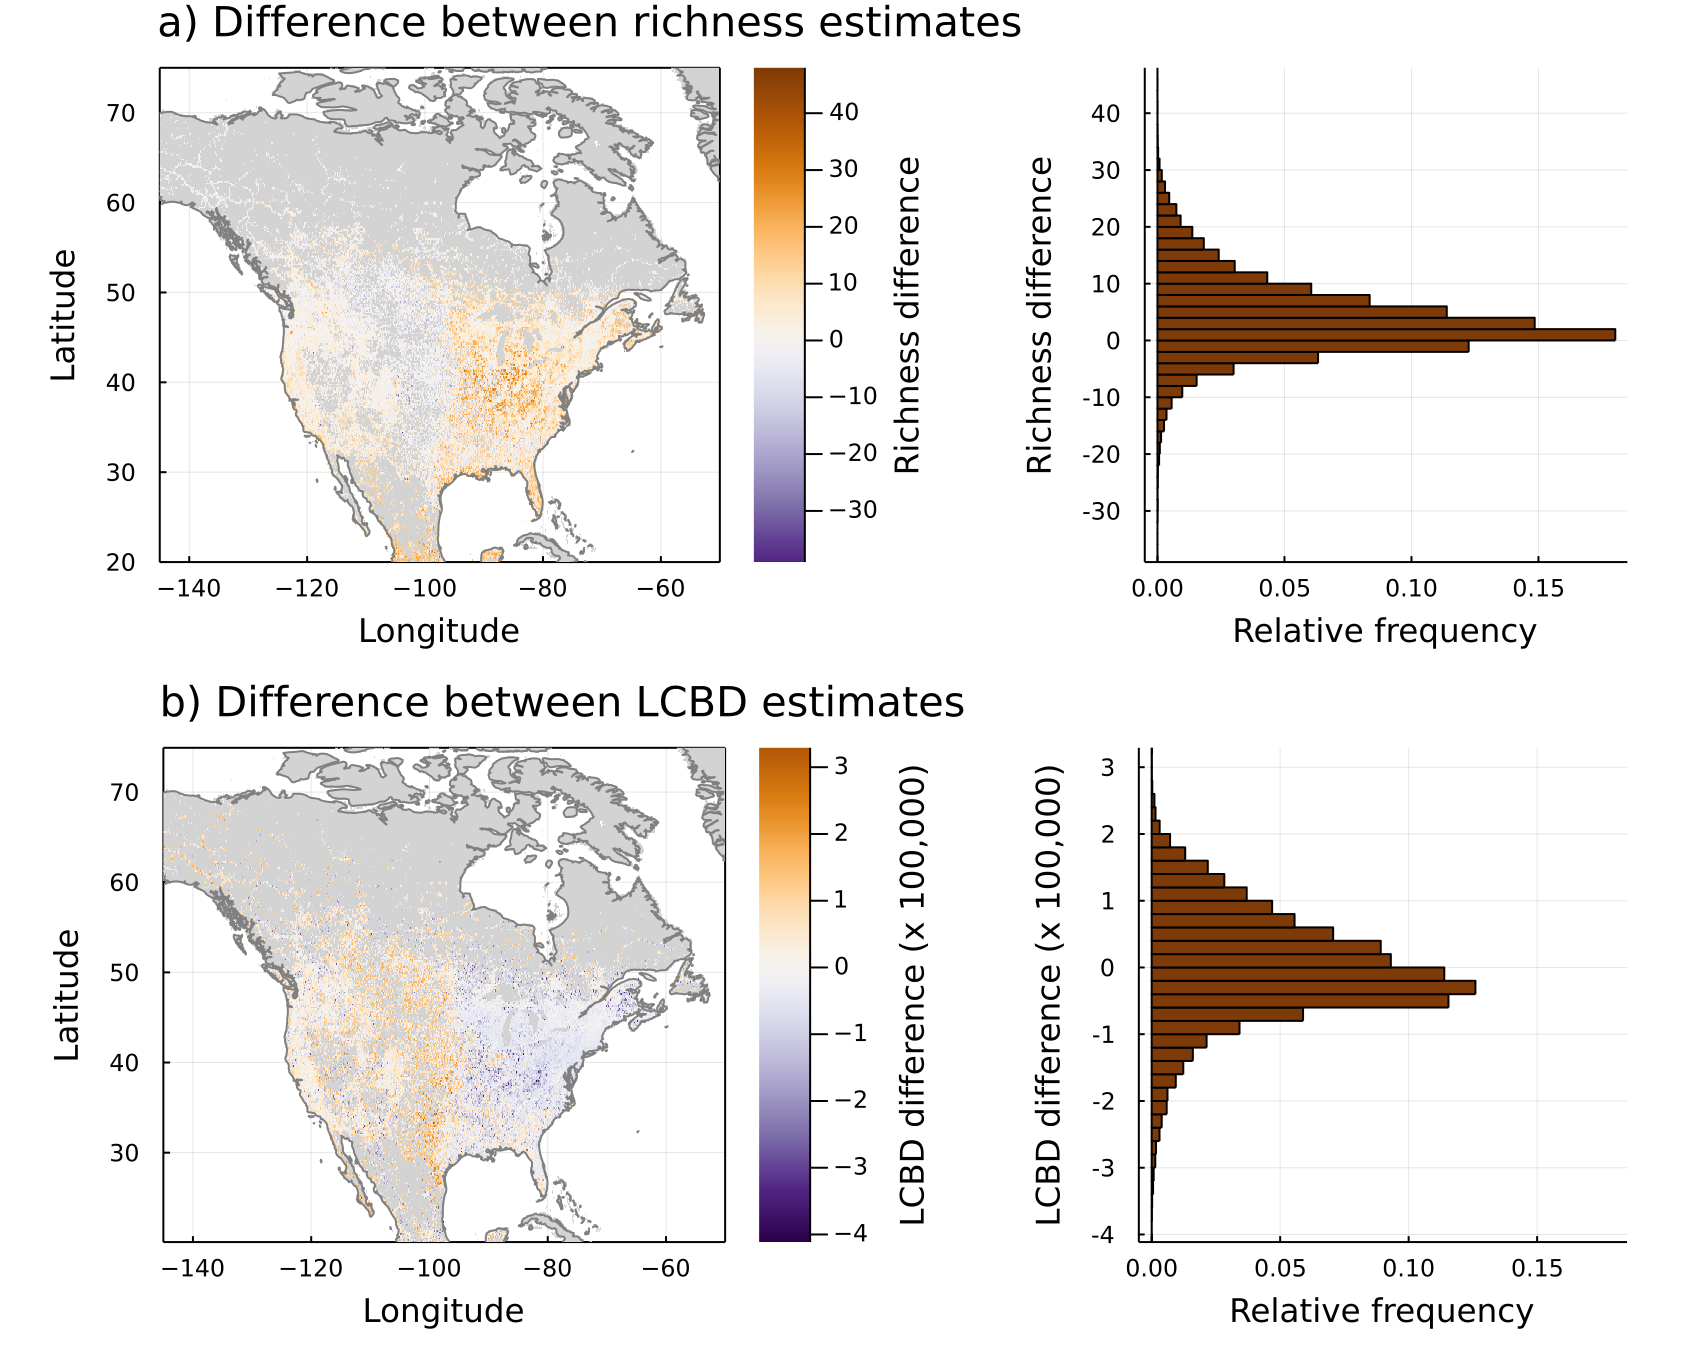
\includegraphics{figures/comparison-difference.png}
\caption{Comparison between observed and predicted estimates of species
richness (a) and ecological uniqueness (b). The difference values
represent the estimate from the predicted data set minus the estimate
from the observed data set. LCBD values were recalculated for the same
set of sites with observations in both data
sets.}\label{fig:comparison-combined}
}
\end{figure}

\begin{figure}
\hypertarget{fig:residuals-combined}{%
\centering
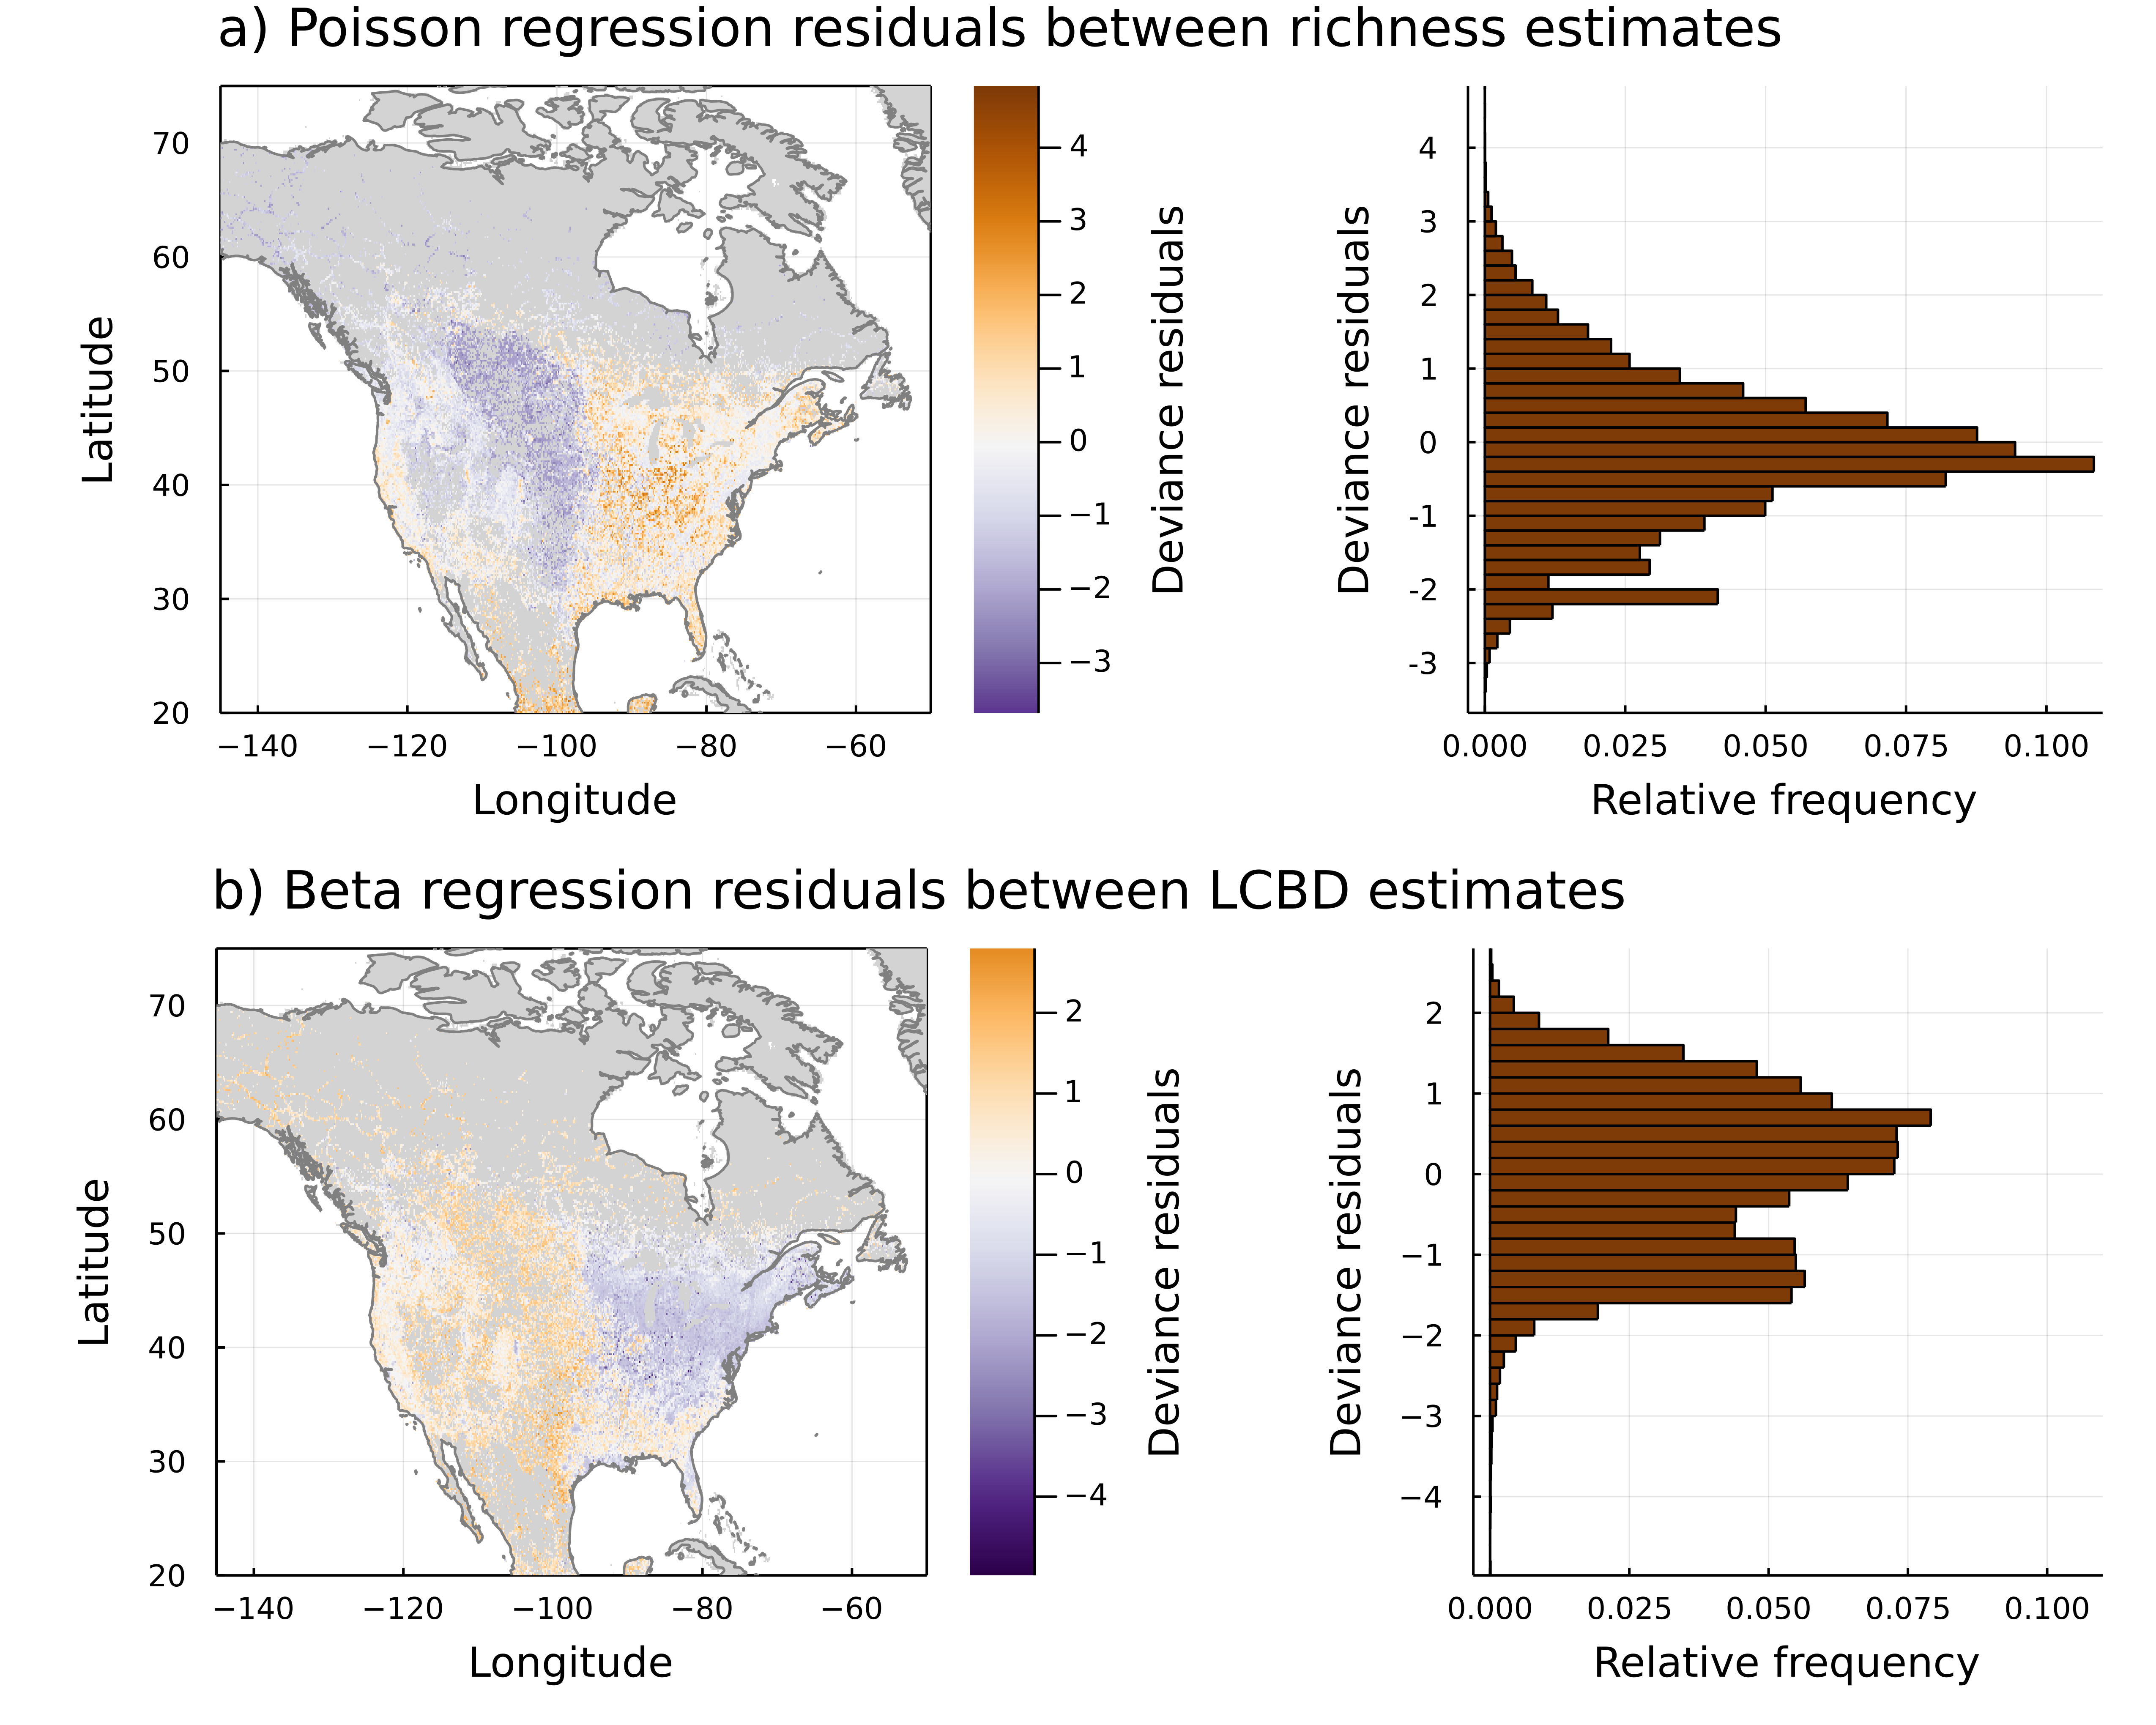
\includegraphics{figures/comparison-residuals.png}
\caption{Comparison of the regression residuals between the observed and
predicted estimates of species richness (a) and ecological uniqueness
(b). The estimate from the predicted data set was used as the dependent
variable and the estimate from the observed data set as the independent
variable. A negative binomial regression with a log link function was
used for species richness, and a beta regression with a logit link
function was used for uniqueness. LCBD values were recalculated for the
same set of sites with observations in both data
sets.}\label{fig:residuals-combined}
}
\end{figure}

\hypertarget{uniqueness-displays-regional-variation-as-two-distinct-profiles}{%
\subsection{Uniqueness displays regional variation as two distinct
profiles}\label{uniqueness-displays-regional-variation-as-two-distinct-profiles}}

The relationship between LCBD values and species richness displayed
contrasting profiles in species-rich and species-poor regions
(Fig.~\ref{fig:subareas}). In the species-rich Northeast region , LCBD
scores displayed a mostly decreasing relationship with species richness,
with a slightly curvilinear form and increase of values for very rich
sites. The sites with the highest LCBD values were the species-poor
sites while the species-rich sites displayed scores. The Southwest
subarea showed a different relationship with a sharper initial decline
and a larger increase as richness reached 20 species. The sites with the
highest LCBD values were the poorest in terms of species richness, as in
the Northeast region, but the species-rich sites were proportionally
more unique in the Southwest region. Total beta diversity was higher in
the Southwest subregion (0.417) than in the Northeast (0.179),
indicating higher compositional differences between the sites.

\begin{figure}
\hypertarget{fig:subareas}{%
\centering
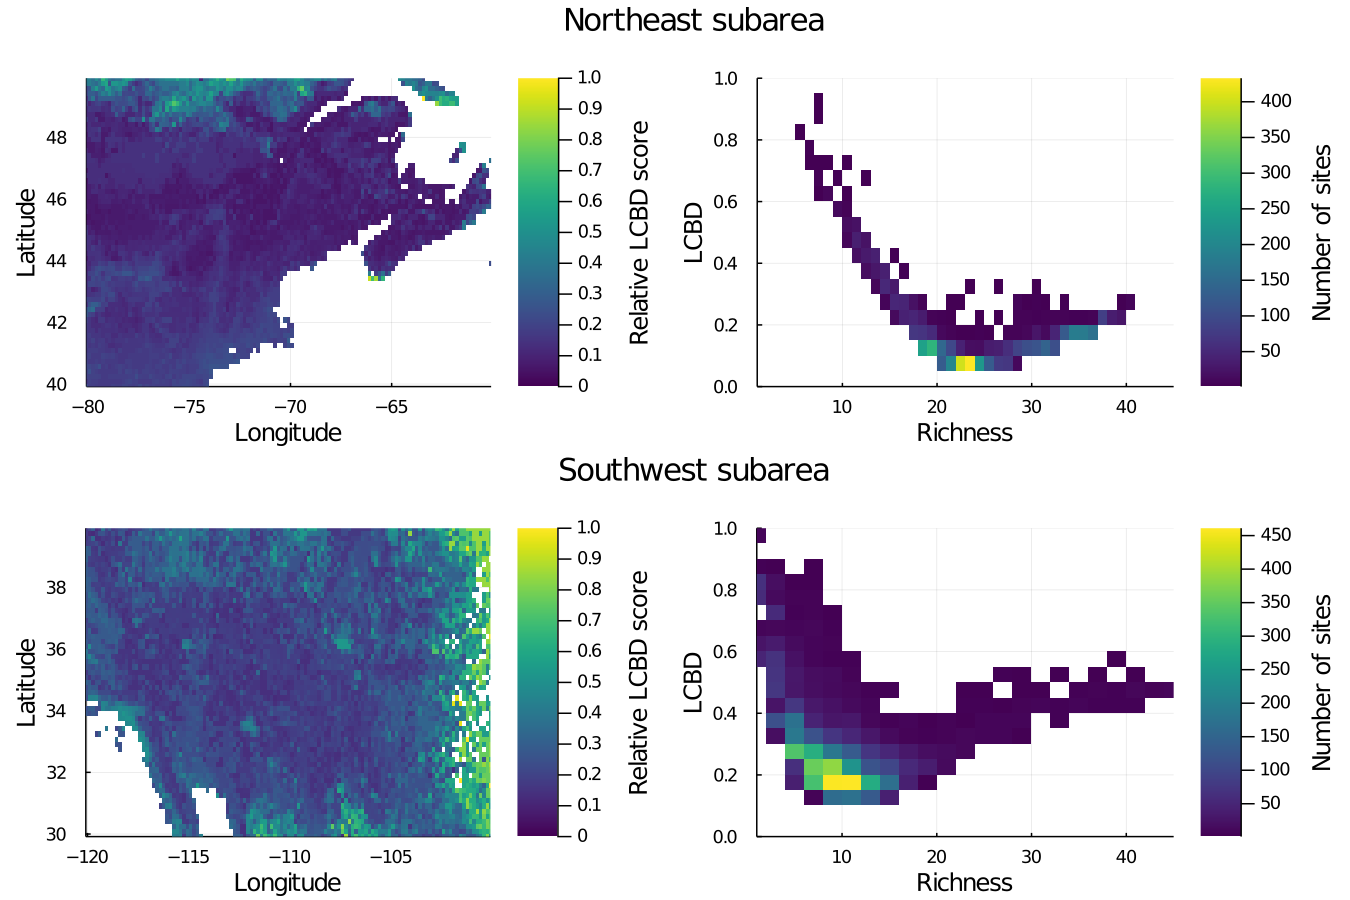
\includegraphics{figures/subareas-combined.png}
\caption{Comparison between a species-rich region (Northeast, a) and a
species-poor one (Southwest, b) based on the SDM predictions for warbler
species in North America. The left-side figures represent the LCBD
scores for the assembled presence-absence predictions, calculated
separately in each region. The colour scales are set to the respective
range of LCBD scores to highlight the relative change within each region
rather than compare the scores between both regions. The right-side
2-dimensional histograms represent the decreasing and slightly
curvilinear relationship between LCBD values and species richness. The
vertical and horizontal dashed lines respectively represent the median
richness and LCBD value in each region, while BDtot represents the total
beta diversity.}\label{fig:subareas}
}
\end{figure}

\hypertarget{uniqueness-depends-on-the-scale-on-which-it-is-measured}{%
\subsection{Uniqueness depends on the scale on which it is
measured}\label{uniqueness-depends-on-the-scale-on-which-it-is-measured}}

The LCBD-richness relationship showed important variation when scaling
up and changing the region's extent (Fig.~\ref{fig:extents}). For
smaller extents, starting with a species-rich region, the relationship
is well defined, mostly decreasing but notably curvilinear (with a
lesser increase for richness values higher than the median). However, as
the extent increases and progressively reaches species-poor regions, the
relationship broadens, displays more variance, and loses its curvilinear
aspect while keeping a decreasing form. Total beta diversity was higher
when increasing the spatial extent, going from 0.121 to 0.284 and 0.687.

\begin{figure}
\hypertarget{fig:extents}{%
\centering
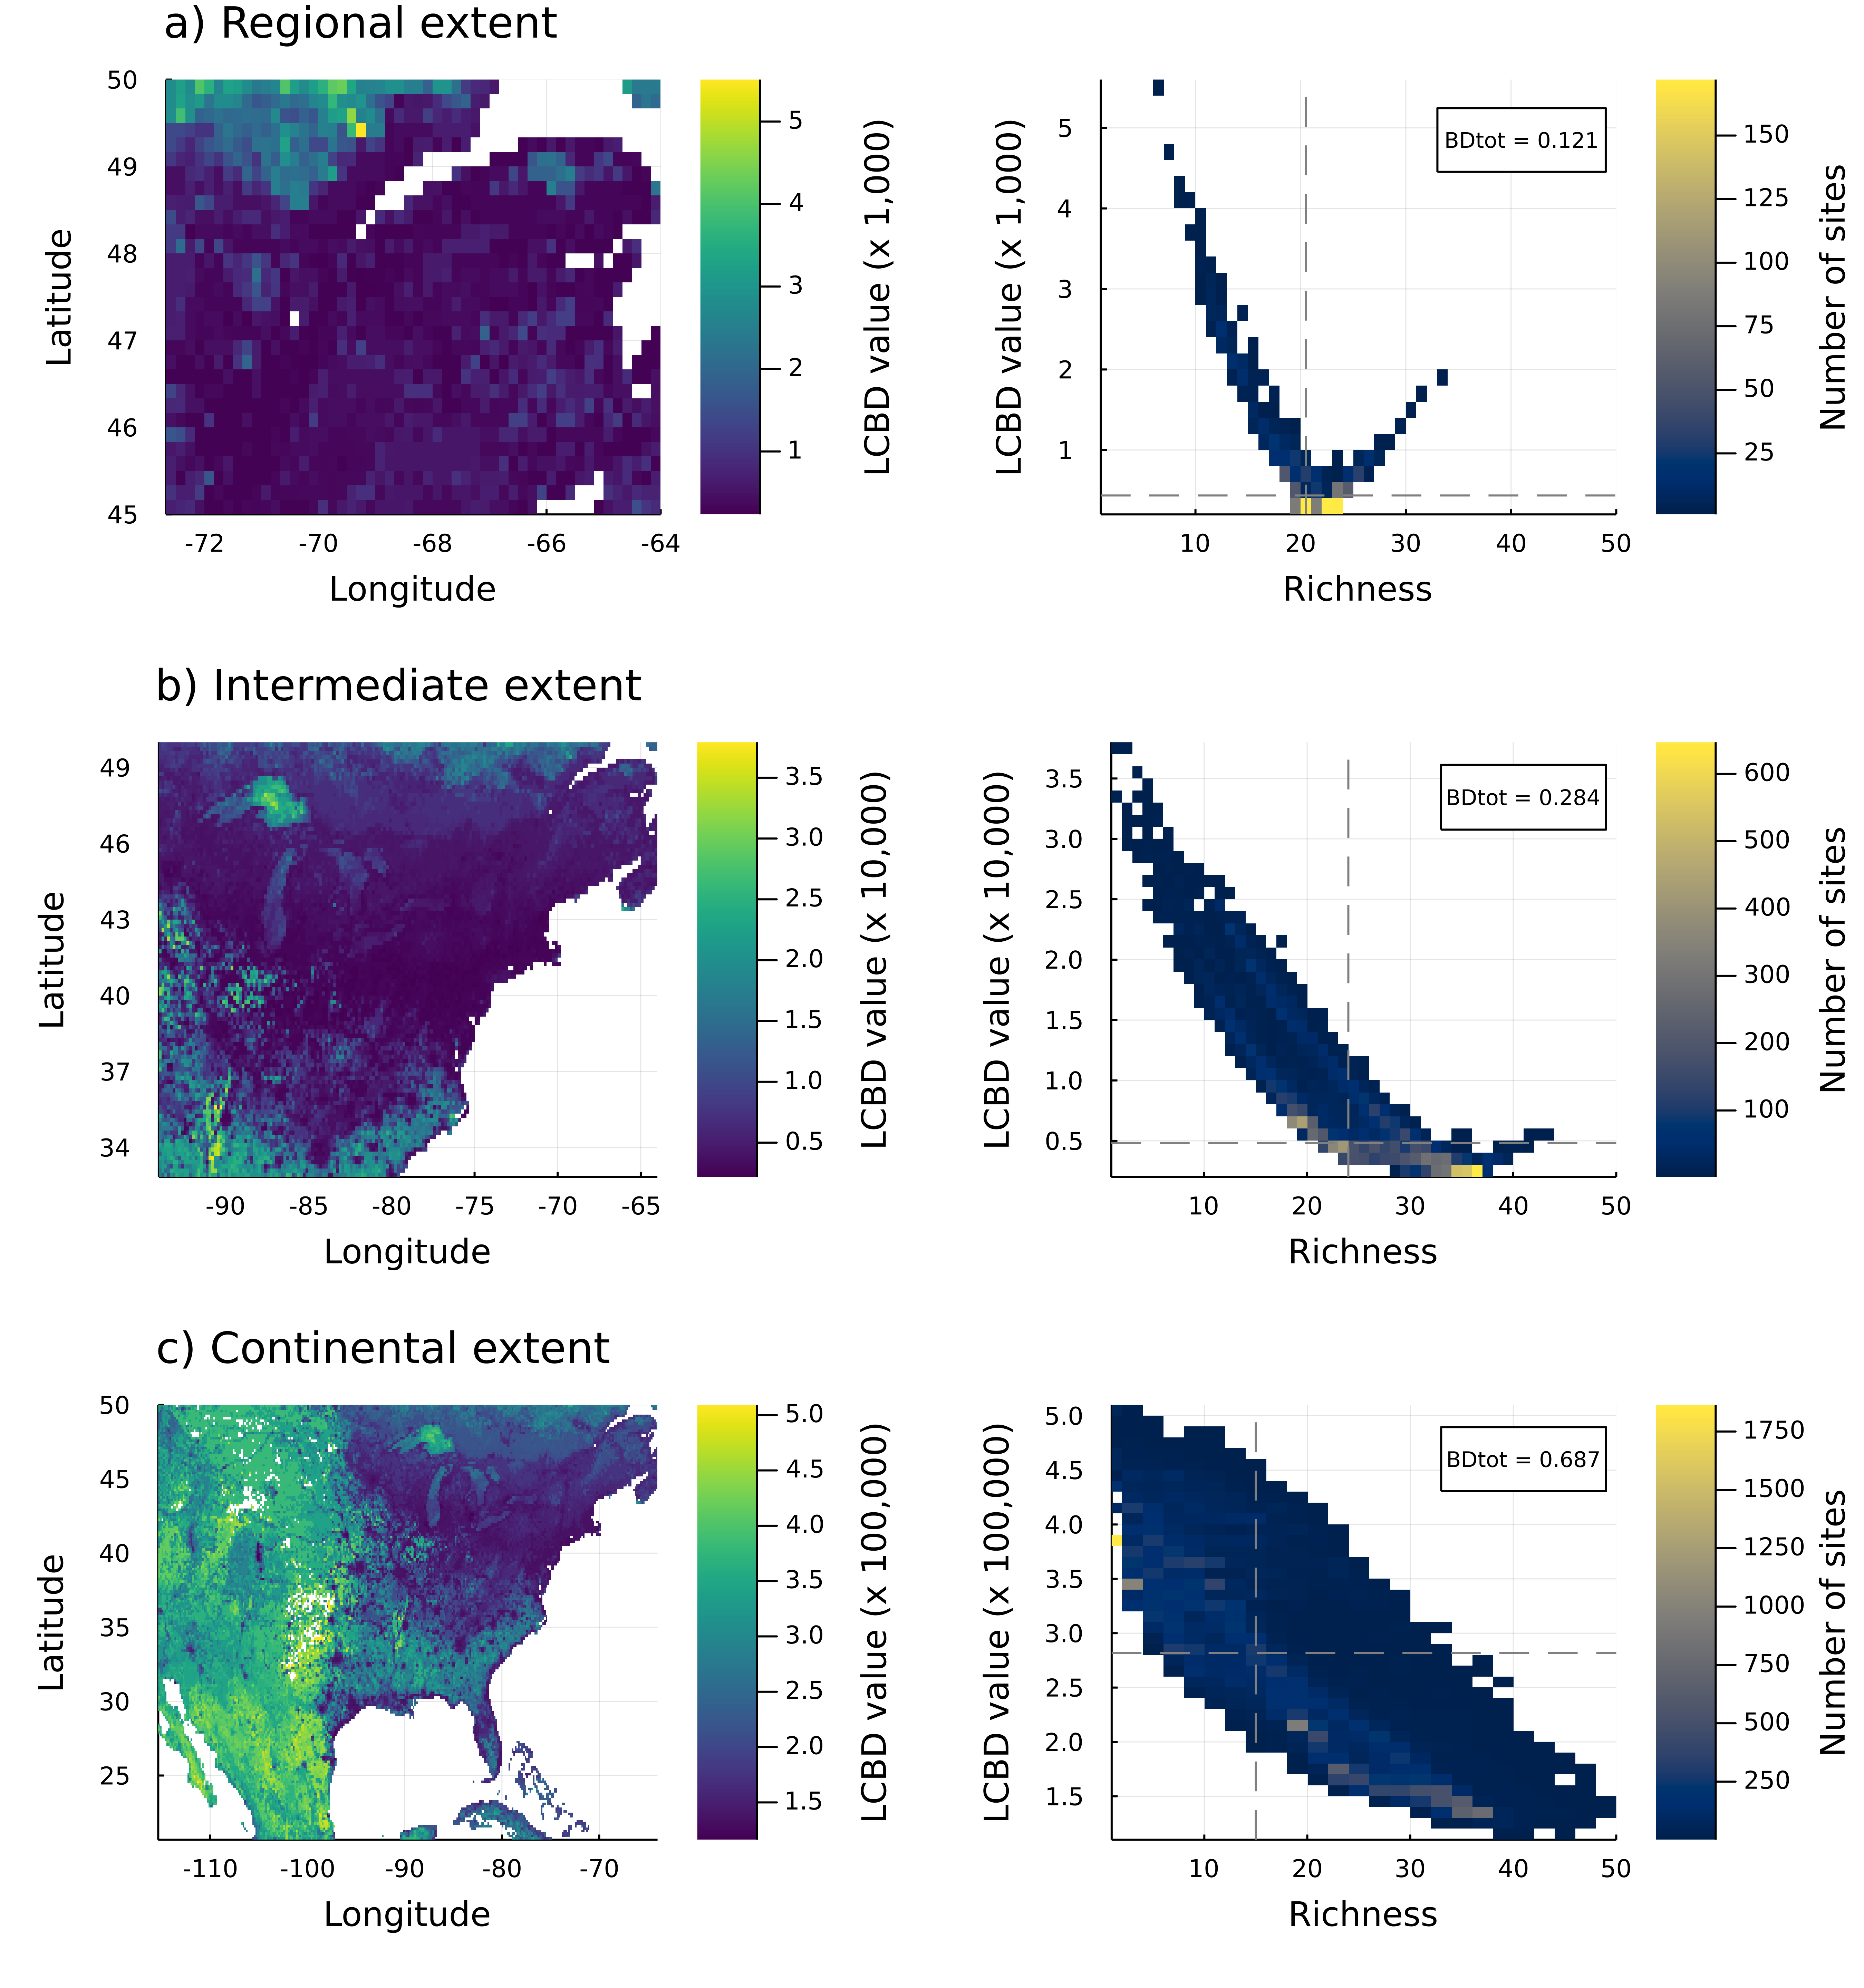
\includegraphics{figures/subareas-extents.png}
\caption{Effect of extent size on the relationship between site richness
and LCBD values based on the SDM predictions for warbler species in
North America. The relationship progressively broadens and displays more
variance when scaling up while total beta diversity increases. The LCBD
values were recalculated at each scale based on the sites in this
region. The vertical and horizontal dashed lines respectively represent
the median richness and LCBD value in each region, while BDtot
represents the total beta diversity.}\label{fig:extents}
}
\end{figure}

\hypertarget{uniqueness-depends-on-the-proportion-of-rare-species}{%
\subsection{Uniqueness depends on the proportion of rare
species}\label{uniqueness-depends-on-the-proportion-of-rare-species}}

The proportion of rare species per site differed depending on the
classification in the ascending or descending portions of the
LCBD-richness relationship (Fig.~\ref{fig:rarespecies}). The proportion
of rare species was higher in the sites corresponding to the ascending
portions of the relationships (shown in \ref{fig:subareas}) than in the
sites corresponding to the descending portions for both subregions. The
classification of the sites in the two portions showed a clear
latitudinal gradient in the Northeast subregion, while it was
distributed in patches in the Southwest subregion
(Fig.~\ref{fig:rarespecies}).

\begin{figure}
\hypertarget{fig:rarespecies}{%
\centering
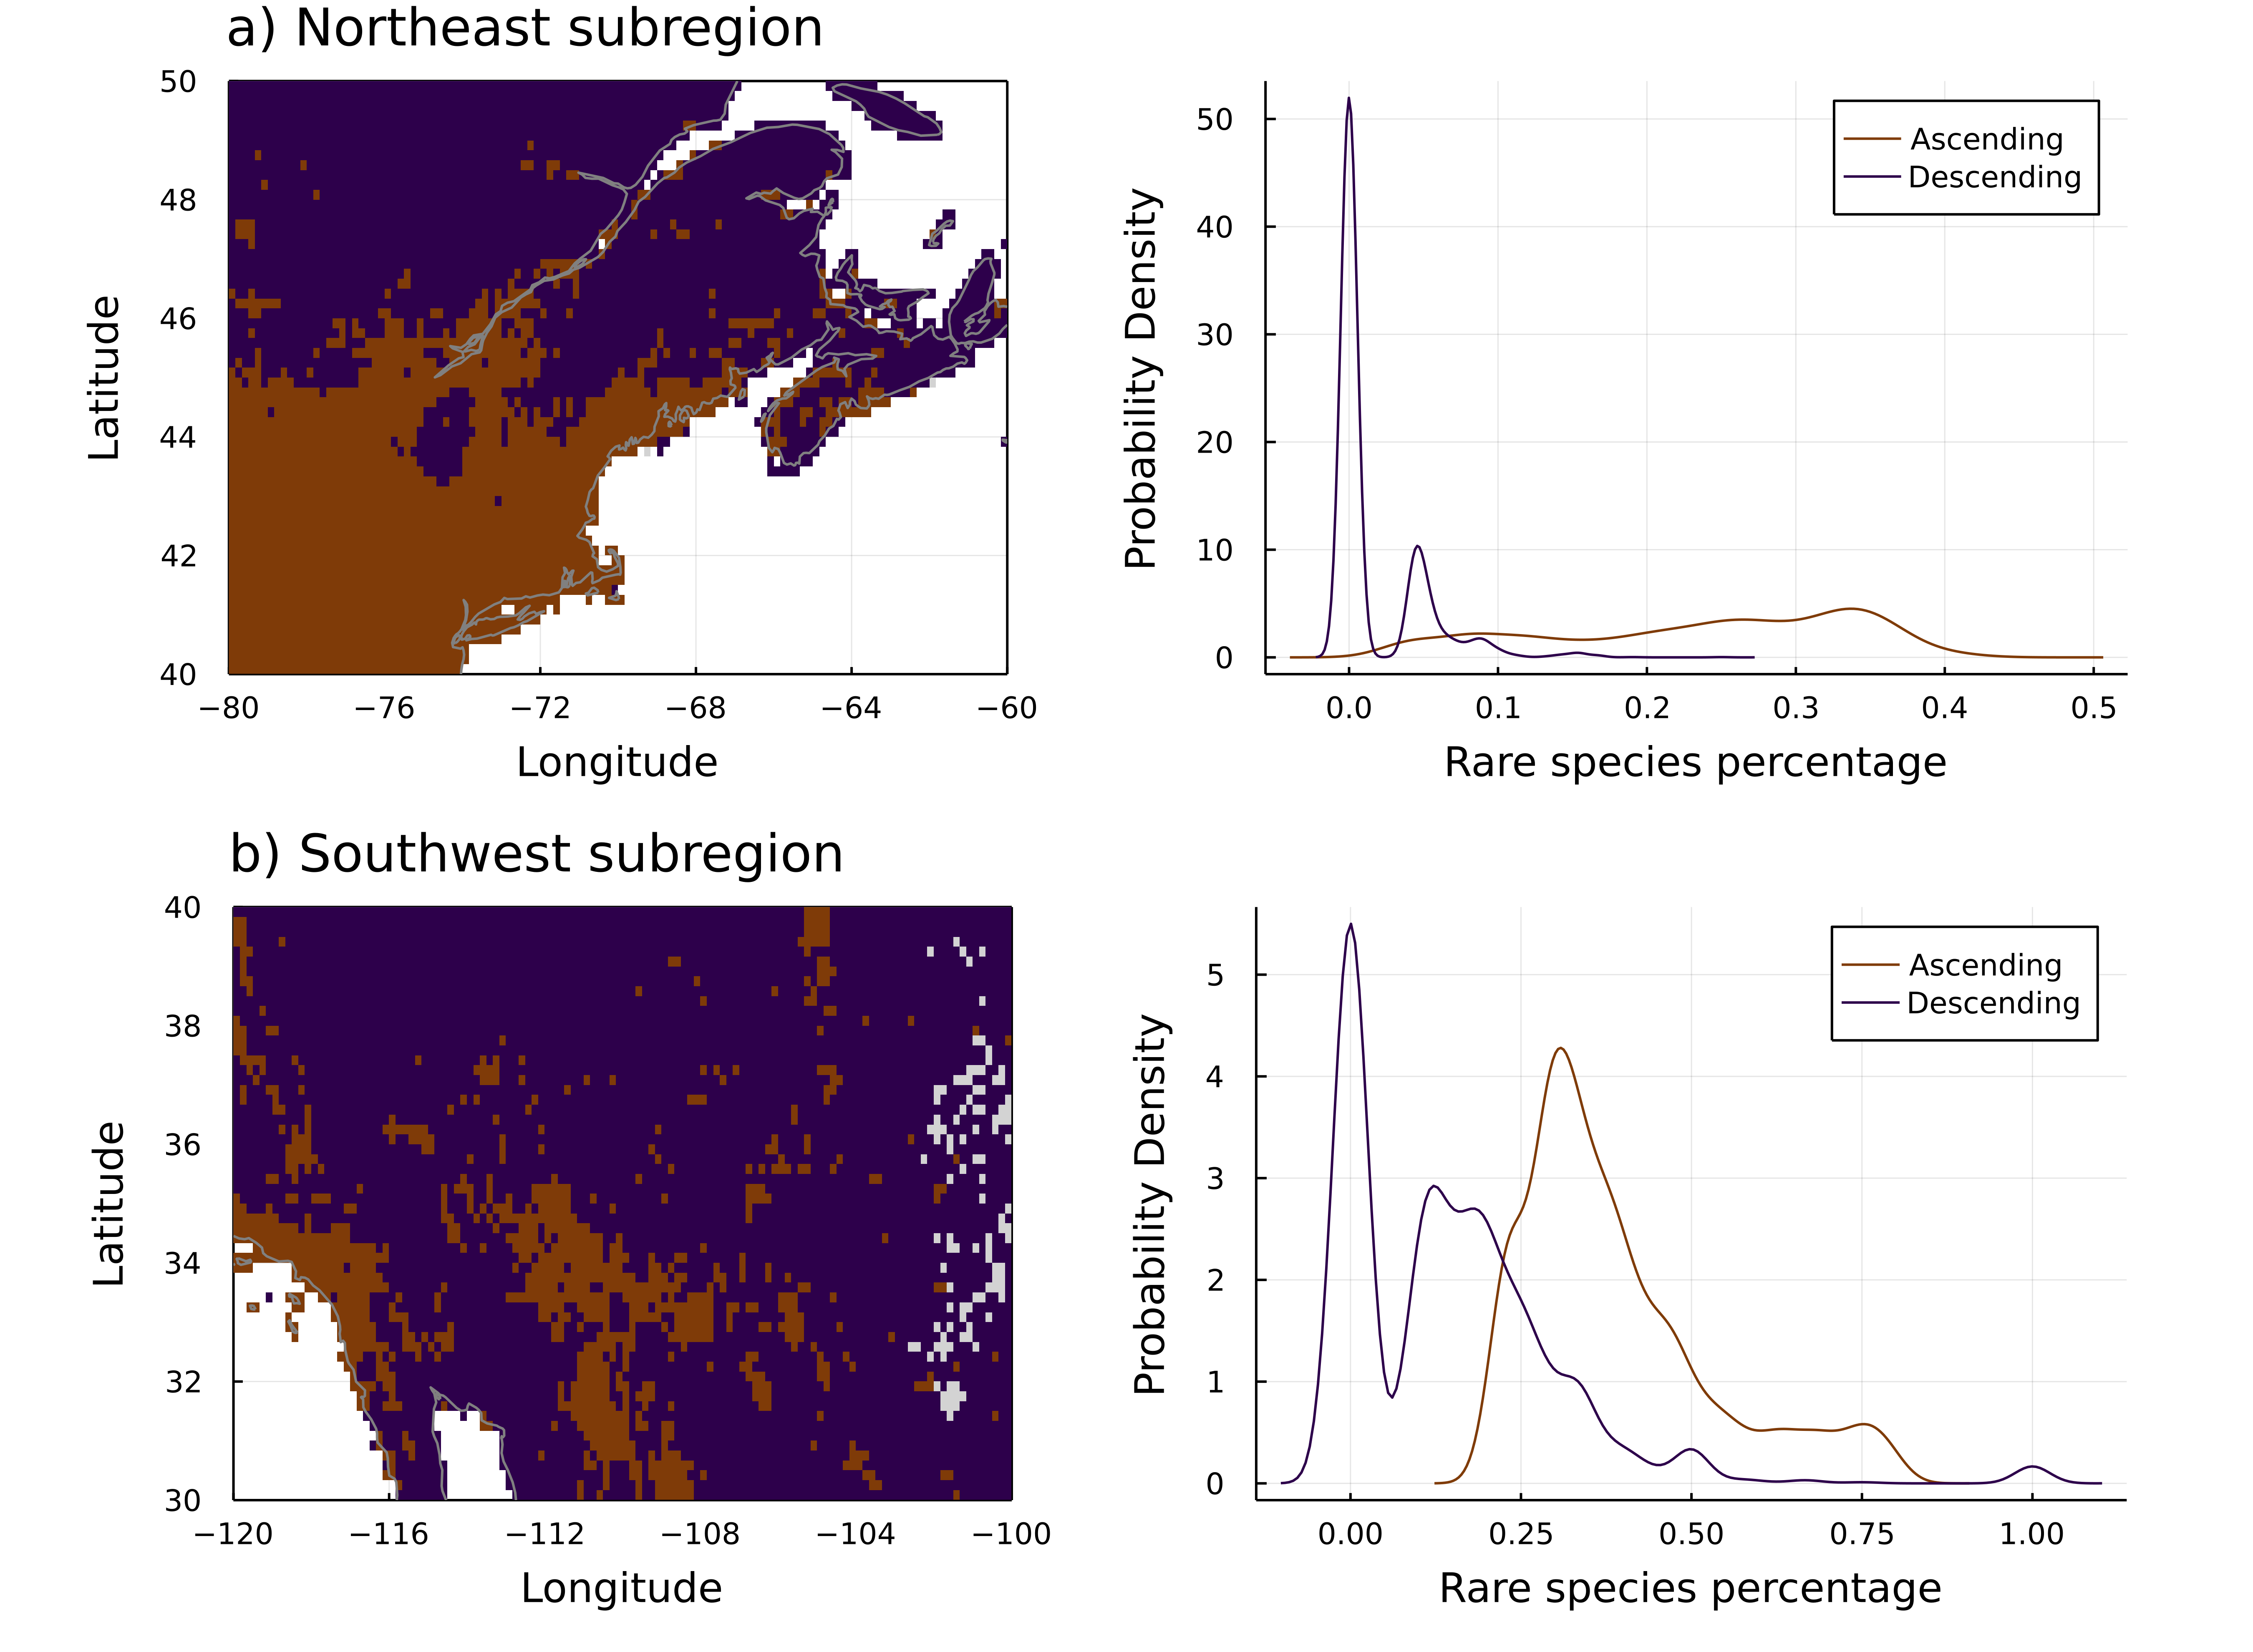
\includegraphics{figures/rare-species.png}
\caption{Proportion of rare species in the ascending and descending
portions of the LCBD-richness relationship for the Northeast (a) and
Southwest (b) subregions. The left side figures show the geographic
distribution of the sites from each group. Sites were assigned to the
ascending portion if their species richness was higher than the richness
of the site with the lowest LCBD value, which corresponds to the
inflection point of the right side figures of Fig.~\ref{fig:subareas},
and in the descending portion otherwise. The right side figures
represent the kernel density estimation of the proportion of rare
species in each group. Values on the y-axis are probability densities
scaled so that the area under the curve equals one. Similarly, the area
under the curve for a given range of values on the x-axis (proportions
of rare species) represents the probability of observing a value in that
range. Species were classified as rare when they occurred in fewer than
40\% of the sites in the subregion. The proportion of rare species was
then calculated for every site.}\label{fig:rarespecies}
}
\end{figure}

\hypertarget{discussion}{%
\section{Discussion}\label{discussion}}

Our results showed a decreasing relationship between species richness
and LCBD values on broad spatial extents (Fig.~\ref{fig:extents}c) but
also highlighted that the exact form of this relationship varies
depending on the region and the spatial extent on which it is measured.
Our species-rich Northeast subregion (Fig.~\ref{fig:subareas}a) showed a
decreasing relationship, very similar to previous studies, and slightly
curvilinear, as described by Heino and Grönroos (2017) and Tan et al.
(2019). This result for warbler species is in line with the original
study on fish communities (Legendre and De Cáceres 2013) and with
following ones on insect metacommunities (da Silva and Hernández 2014;
Heino et al. 2017; Heino and Grönroos 2017), dung beetles (da Silva,
Hernández, and Heino 2018; da Silva, Bogoni, and Heino 2020), aquatic
beetles (Heino and Alahuhta 2019), stream macroinvertebrates (Sor,
Legendre, and Lek 2018), stream diatoms (Vilmi, Karjalainen, and Heino
2017), multi-trophic pelagic food webs (phytoplankton, zooplankton,
fish) (Taranu, Pinel-Alloul, and Legendre 2020), temperate forest trees
(Tan et al. 2019), mammals (da Silva, Bogoni, and Heino 2020), wetland
birds (de Deus et al. 2020), and various phylogenetic groups (plants,
lizards, mites, anurans, mesoinvertebrates) (Landeiro et al. 2018).
However, it was originally argued that the negative relationship was not
general or obligatory (Legendre and De Cáceres 2013). Different
LCBD-richness relationships have also been observed, with both positive
and negative relationships for different sites or taxonomic groups in
some studies (Kong et al. 2017; Teittinen et al. 2017), as well as a
negative relationship with the number of common species but a positive
relationship with the number of rare species (Qiao et al. 2015).

Our results further show that the relationship may depend on the
region's richness profile, as the relationship was different in our
species-poor Southwest subregion, with a sharper initial decrease
(Fig.~\ref{fig:subareas}b). Therefore, the curvilinear form may depend
on how pronounced the contrast is between the region's median richness
and its richest ecologically feasible sites. The increasing part of the
curvilinear form for higher richness values was also more pronounced in
our results (Fig.~\ref{fig:subareas}a,b; Fig.~\ref{fig:extents}c) than
in previous studies (e.g, Tan et al. 2019), which reinforces the idea
that the relationship and its curvilinear form may vary depending on the
region.

The variation in the LCBD-richness relationship when extending the study
extent showed that the uniqueness patterns highlighted are not
necessarily the same depending on the scale on which it is used
(Fig.~\ref{fig:extents}). The relationship progressively lost its clear
definition and curvilinear form as the East and West profiles merged,
creating a new distinct profile with more variation and no curvilinear
form. Therefore, aggregating too many different sites might possibly
mask some patterns of uniqueness in species-rich sites. Total beta
diversity, on the other hand, showed the variation expected from
previous studies, increasing with spatial extent
(Fig.~\ref{fig:extents}) (Barton et al. 2013; Heino et al. 2015). Its
value was high at the continental scale (0.687) but lower than what has
been observed in some studies (e.g., 0.80 on macroinvertebrate
communities in the Lower Mekong Basin by Sor, Legendre, and Lek 2018).

Our results confirm that the proportion of rare species in the community
may affect the direction of the relationship between species richness
and ecological uniqueness (Fig.~\ref{fig:rarespecies}). da Silva,
Hernández, and Heino (2018) suggested that the proportion of rare and
common species in the communities determines whether the relationship
will be negative, non-significant, or positive. Yao et al. (2021) showed
an association between the direction of the relationship and the
proportion of rare species, with sites with a lower proportion (between
60\% and 75\% in their case) displaying a negative relationship and
sites with a higher proportion (around 85\%) showing a positive one. Our
results further show that sites associated with a positive relationship
within a curvilinear one tended to have a higher rare species proportion
(Fig.~\ref{fig:rarespecies}). This also implies that the proportion of
rare species was higher in species-rich sites than in species-poor ones
in both our Northeast and Southwest subregions. Further work should
attempt to disentangle the effects of the rare species proportion and
the region's richness profile.

Our results showed that SDM models provide richness and uniqueness
predictions highly correlated to the occurrence data while filling gaps
in poorly sampled regions (Fig.~\ref{fig:maps}). The results showed a
statistically significant spatial association between predicted and
observed estimates despite correcting for autocorrelation using the
modified \emph{t}-test from Clifford, Richardson, and Hemon (1989). A
positive autocorrelation on large distances indicates aggregates or
structures repeating through space (Legendre and Fortin 1989). This is
consistent with our results, as the distribution of richness and
uniqueness values was visibly spatially structured in both our observed
and predicted data (Fig.~\ref{fig:maps}). Nonetheless, it is possible
that the autocorrelation in the predicted values could represent an
artifact of the predictive models (capturing the spatial structure from
the environmental variables, for example), and might not represent the
true autocorrelation expected for the uniqueness estimates. Further work
could verify this by quantitatively comparing the autocorrelation and
spatial structures in the observed and predicted uniqueness estimates.

Predicted values also tended to underestimate uniqueness in species-rich
regions and overestimate it in species-poor ones, with the opposite
trend for species richness
(Figs.~\ref{fig:comparison-combined}, \ref{fig:residuals-combined}).
Overprediction of richness using S-SDMs was reported previously (Dubuis
et al. 2011; D'Amen et al. 2015; Zurell et al. 2020). No comparable
baseline exists for predictions of LCBD values, as our study is the
first to compare LCBD estimates from observed and predicted data in such
a way. However, some studies showed that LCBD distributions were
spatially structured across sampling sites (da Silva, Hernández, and
Heino 2018). On the other hand, the spatial structure in our results did
not exactly concord with the one reported by Heino and Alahuhta (2019),
who showed a negative relationship between LCBD values and latitude for
diving beetles communities in Northern Europe. In comparison, our LCBD
scores increased both in the North and South (Fig.~\ref{fig:maps}),
hence did not strictly increase with latitude, and also showed a clear
East-West gradient. Overall, our distribution results
(Figs.~\ref{fig:maps}, \ref{fig:comparison-combined}, \ref{fig:residuals-combined})
also have implications for conservation, as they confirm that species
richness and ecological uniqueness measured from LCBD values may
conflict and highlight different potential hotspots (Dubois, Proulx, and
Pellerin 2020; Yao et al. 2021), thus reinstating the need to protect
both with complementary strategies.

Our predictions for regions with sparse sampling are of interest as they
allow a quantitative evaluation, however imperfect, for sites where we
would otherwise have no information. Our SDMs also offered relevant LCBD
predictions using eBird, arguably one of the largest presence-absence
data sets available (when using its complete checklist system), showing
the measure's potential on such massive data. Together, the potential to
generate uniqueness predictions in new locations and through massive
data opens new opportunities for LCBD analyses on extended spatial
scales and on a broader diversity of taxons. An interesting way forward
would be to test these results using more advanced community assembling
techniques than S-SDMs. The use of SESAM (Guisan and Rahbek 2011) with
probabilistic SDMs, probability ranking, and species richness
predictions as macroecological constraints returns high site-level
prediction accuracy (Zurell et al. 2020) and would be compatible with
presence-absence LCBD calculations. The use of probabilistic stacks
rather than binary ones (Calabrese et al. 2014) could also constitute a
novel way to calculate LCBD indices. Both these procedures should reduce
the richness deviation we observed, and it would be interesting to
verify if this can also be the case with LCBD values. An ensemble of SDM
algorithms could also be used to capture a broader range of possible
outcomes for the LCBD predictions. However, given the high performance
of BARTs in model comparisons (Konowalik and Nosol 2021; Tytar and
Baidashnikov 2021) and the large extent we covered, we do not believe
the changes to the LCBD gradients would be strong enough to affect our
results in a meaningful way.

This study showed how ecological uniqueness can be measured over broad
spatial extents, including for regions with sparse sampling, and how
scale changes may affect beta diversity quantification. It is the first
study to assess the relevance of local contributions to beta diversity
calculated on the output of species distribution models. It is also the
first to compare the relationship between LCBD values and species
richness for different regions and spatial extents. First, our results
showed that the negative relationship often observed between species
richness and LCBD scores can take different forms depending on the
richness profile of the regions on which it is measured. Therefore,
species-rich and species-poor regions may display different ways to be
unique. Second, the negative relationship was not constant when varying
the spatial study extent and may be less clearly defined at broad scales
when contrasting regional relationships are present. The broad-scale
uniqueness profile might then be completely distinct from the regional
profiles constituting it. Finally, species distribution models offer a
promising way to generate uniqueness predictions on broad spatial
extents and could prove useful to identify beta diversity hotspots in
unsampled locations on large spatial scales, which could be important
targets for conservation purposes.

\hypertarget{acknowledgments}{%
\section{Acknowledgments}\label{acknowledgments}}

We acknowledge that this study was conducted on land within the
traditional unceded territory of the Saint Lawrence Iroquoian,
Anishinabewaki, Mohawk, Huron-Wendat, and Omàmiwininiwak nations. We
received financial support from the Fonds de recherche du Québec -
Nature et technologie (FRQNT) and the Computational Biodiversity Science
and Services (BIOS\textsuperscript{2}) NSERC CREATE training program. We
thank Élise Filotas and Anne-Lise Routier for their helpful comments on
this manuscript.

\hypertarget{references}{%
\section*{References}\label{references}}
\addcontentsline{toc}{section}{References}

\hypertarget{refs}{}
\begin{CSLReferences}{1}{0}
\leavevmode\hypertarget{ref-Barton2013SpaSca}{}%
Barton, Philip S., Saul A. Cunningham, Adrian D. Manning, Heloise Gibb,
David B. Lindenmayer, and Raphael K. Didham. 2013. {``The Spatial
Scaling of Beta Diversity.''} \emph{Global Ecology and Biogeography} 22
(6): 639--47. \url{https://doi.org/10.1111/geb.12031}.

\leavevmode\hypertarget{ref-Bezanson2017JulFre}{}%
Bezanson, Jeff, Alan Edelman, Stefan Karpinski, and Viral B. Shah. 2017.
{``Julia: A Fresh Approach to Numerical Computing.''} \emph{SIAM Review}
59 (1): 65--98. \url{https://doi.org/10.1137/141000671}.

\leavevmode\hypertarget{ref-Booth2014BioFir}{}%
Booth, Trevor H., Henry A. Nix, John R. Busby, and Michael F.
Hutchinson. 2014. {``BIOCLIM: The First Species Distribution Modelling
Package, Its Early Applications and Relevance to Most Current MaxEnt
Studies.''} \emph{Diversity and Distributions} 20 (1): 1--9.
\url{https://doi.org/10.1111/ddi.12144}.

\leavevmode\hypertarget{ref-Buchhorn2019CopGlo}{}%
Buchhorn, Marcel, Bruno Smets, Luc Bertels, Myroslava Lesiv,
Nandin-Erdene Tsendbazar, Martin Herold, and Steffen Fritz. 2019.
{``Copernicus Global Land Service: Land Cover 100m: Epoch 2015:
Globe.''} Zenodo. \url{https://doi.org/10.5281/zenodo.3243509}.

\leavevmode\hypertarget{ref-Calabrese2014StaSpe}{}%
Calabrese, Justin M., Grégoire Certain, Casper Kraan, and Carsten F.
Dormann. 2014. {``Stacking Species Distribution Models and Adjusting
Bias by Linking Them to Macroecological Models.''} \emph{Global Ecology
and Biogeography} 23 (1): 99--112.
\url{https://doi.org/10.1111/geb.12102}.

\leavevmode\hypertarget{ref-Carlson2020EmbSpe}{}%
Carlson, Colin J. 2020. {``Embarcadero: Species Distribution Modelling
with Bayesian Additive Regression Trees in R.''} \emph{Methods in
Ecology and Evolution} 11 (7): 850--58.
\url{https://doi.org/10.1111/2041-210X.13389}.

\leavevmode\hypertarget{ref-Chipman2010BarBay}{}%
Chipman, Hugh A., Edward I. George, and Robert E. McCulloch. 2010.
{``BART: Bayesian Additive Regression Trees.''} \emph{Annals of Applied
Statistics} 4 (1): 266--98. \url{https://doi.org/10.1214/09-AOAS285}.

\leavevmode\hypertarget{ref-Clifford1989AssSig}{}%
Clifford, Peter, Sylvia Richardson, and Denis Hemon. 1989. {``Assessing
the Significance of the Correlation Between Two Spatial Processes.''}
\emph{Biometrics} 45 (1): 123--34.
\url{https://doi.org/10.2307/2532039}.

\leavevmode\hypertarget{ref-CommissionforEnvironmentalCooperation1997EcoReg}{}%
Commission for Environmental Cooperation. 1997. \emph{Ecological Regions
of North America}. Commission for Environmental Cooperation.
\url{http://www3.cec.org/islandora/en/item/1701-ecological-regions-north-america-toward-common-perspective/}.

\leavevmode\hypertarget{ref-Cribari-Neto2010BetReg}{}%
Cribari-Neto, Francisco, and Achim Zeileis. 2010. {``Beta Regression in
R.''} \emph{Journal of Statistical Software} 34 (1): 1--24.
\url{https://doi.org/10.18637/jss.v034.i02}.

\leavevmode\hypertarget{ref-DAmen2015UsiSpe}{}%
D'Amen, Manuela, Anne Dubuis, Rui F. Fernandes, Julien Pottier, Loïc
Pellissier, and Antoine Guisan. 2015. {``Using Species Richness and
Functional Traits Predictions to Constrain Assemblage Predictions from
Stacked Species Distribution Models.''} \emph{Journal of Biogeography}
42 (7): 1255--66. \url{https://doi.org/10.1111/jbi.12485}.

\leavevmode\hypertarget{ref-DAntraccoli2020MorSpe}{}%
D'Antraccoli, Marco, Giovanni Bacaro, Enrico Tordoni, Gianni Bedini, and
Lorenzo Peruzzi. 2020. {``More Species, Less Effort: Designing and
Comparing Sampling Strategies to Draft Optimised Floristic
Inventories.''} \emph{Perspectives in Plant Ecology, Evolution and
Systematics} 45: 125547.
\url{https://doi.org/10.1016/j.ppees.2020.125547}.

\leavevmode\hypertarget{ref-Dansereau2021SimJl}{}%
Dansereau, Gabriel, and Timothée Poisot. 2021. {``SimpleSDMLayers.jl and
GBIF.jl: A Framework for Species Distribution Modeling in Julia.''}
\emph{Journal of Open Source Software} 6 (57): 2872.
\url{https://doi.org/10.21105/joss.02872}.

\leavevmode\hypertarget{ref-DeCaceres2012VarTre}{}%
De Cáceres, Miquel, Pierre Legendre, Renato Valencia, Min Cao, Li-Wan
Chang, George Chuyong, Richard Condit, et al. 2012. {``The Variation of
Tree Beta Diversity Across a Global Network of Forest Plots.''}
\emph{Global Ecology and Biogeography} 21 (12): 1191--1202.
\url{https://doi.org/10.1111/j.1466-8238.2012.00770.x}.

\leavevmode\hypertarget{ref-deDeus2020AviBet}{}%
Deus, Filipe Ferreira de, Karl-L. Schuchmann, Julia Arieira, Ana Silvia
de Oliveira Tissiani, and Marinêz Isaac Marques. 2020. {``Avian Beta
Diversity in a Neotropical Wetland: The Effects of Flooding and
Vegetation Structure.''} \emph{Wetlands} 40 (5): 1513--27.
\url{https://doi.org/10.1007/s13157-019-01240-0}.

\leavevmode\hypertarget{ref-Dray2021AdeMul}{}%
Dray, Stéphane, David Bauman, Guillaume Blanchet, Daniel Borcard, Sylvie
Clappe, Guillaume Guenard, Thibaut Jombart, et al. 2021. {``Adespatial:
Multivariate Multiscale Spatial Analysis.''}
\url{https://CRAN.R-project.org/package=adespatial}.

\leavevmode\hypertarget{ref-Dubois2020EcoUni}{}%
Dubois, Raphaëlle, Raphaël Proulx, and Stéphanie Pellerin. 2020.
{``Ecological Uniqueness of Plant Communities as a Conservation
Criterion in Lake-Edge Wetlands.''} \emph{Biological Conservation} 243:
108491. \url{https://doi.org/10.1016/j.biocon.2020.108491}.

\leavevmode\hypertarget{ref-Dubuis2011PreSpa}{}%
Dubuis, Anne, Julien Pottier, Vanessa Rion, Loïc Pellissier, Jean-Paul
Theurillat, and Antoine Guisan. 2011. {``Predicting Spatial Patterns of
Plant Species Richness: A Comparison of Direct Macroecological and
Species Stacking Modelling Approaches.''} \emph{Diversity and
Distributions} 17 (6): 1122--31.
\url{https://doi.org/10.1111/j.1472-4642.2011.00792.x}.

\leavevmode\hypertarget{ref-eBirdBasicDataset2019VerEbd}{}%
eBird Basic Dataset. 2019. \emph{Version: EBD\_relJun-2019}. Cornell Lab
of Ornithology, Ithaca, NY, USA.

\leavevmode\hypertarget{ref-Ferrier2006SpaMod}{}%
Ferrier, Simon, and Antoine Guisan. 2006. {``Spatial Modelling of
Biodiversity at the Community Level.''} \emph{Journal of Applied
Ecology} 43 (3): 393--404.
\url{https://doi.org/10.1111/j.1365-2664.2006.01149.x}.

\leavevmode\hypertarget{ref-Fick2017Wor2N}{}%
Fick, Stephen E., and Robert J. Hijmans. 2017. {``WorldClim 2: New 1-Km
Spatial Resolution Climate Surfaces for Global Land Areas.''}
\emph{International Journal of Climatology} 37 (12): 4302--15.
\url{https://doi.org/10.1002/joc.5086}.

\leavevmode\hypertarget{ref-GDALux2fOGRcontributors2021GdaOgr}{}%
GDAL/OGR contributors. 2021. \emph{GDAL/OGR Geospatial Data Abstraction
Software Library}. Manual. Open Source Geospatial Foundation.
\url{https://gdal.org}.

\leavevmode\hypertarget{ref-Guisan2011SesNew}{}%
Guisan, Antoine, and Carsten Rahbek. 2011. {``SESAM a New Framework
Integrating Macroecological and Species Distribution Models for
Predicting Spatio-Temporal Patterns of Species Assemblages.''}
\emph{Journal of Biogeography} 38 (8): 1433--44.
\url{https://doi.org/10.1111/j.1365-2699.2011.02550.x}.

\leavevmode\hypertarget{ref-Guisan2005PreSpe}{}%
Guisan, Antoine, and Wilfried Thuiller. 2005. {``Predicting Species
Distribution: Offering More Than Simple Habitat Models.''} \emph{Ecology
Letters} 8 (9): 993--1009.
\url{https://doi.org/10.1111/j.1461-0248.2005.00792.x}.

\leavevmode\hypertarget{ref-Heino2019KniPat}{}%
Heino, Jani, and Janne Alahuhta. 2019. {``Knitting Patterns of
Biodiversity, Range Size and Body Size in Aquatic Beetle Faunas:
Significant Relationships but Slightly Divergent Drivers.''}
\emph{Ecological Entomology} 44 (3): 413--24.
\url{https://doi.org/10.1111/een.12717}.

\leavevmode\hypertarget{ref-Heino2017UnrCor}{}%
Heino, Jani, Luis Mauricio Bini, Johan Andersson, Johannes Bergsten, Ulf
Bjelke, and Frank Johansson. 2017. {``Unravelling the Correlates of
Species Richness and Ecological Uniqueness in a Metacommunity of Urban
Pond Insects.''} \emph{Ecological Indicators} 73: 422--31.
\url{https://doi.org/10.1016/j.ecolind.2016.10.006}.

\leavevmode\hypertarget{ref-Heino2017ExpSpe}{}%
Heino, Jani, and Mira Grönroos. 2017. {``Exploring Species and Site
Contributions to Beta Diversity in Stream Insect Assemblages.''}
\emph{Oecologia} 183 (1): 151--60.
\url{https://doi.org/10.1007/s00442-016-3754-7}.

\leavevmode\hypertarget{ref-Heino2015ComAna}{}%
Heino, Jani, Adriano S. Melo, Luis Mauricio Bini, Florian Altermatt,
Salman A. Al-Shami, David G. Angeler, Núria Bonada, et al. 2015. {``A
Comparative Analysis Reveals Weak Relationships Between Ecological
Factors and Beta Diversity of Stream Insect Metacommunities at Two
Spatial Levels.''} \emph{Ecology and Evolution} 5 (6): 1235--48.
\url{https://doi.org/10.1002/ece3.1439}.

\leavevmode\hypertarget{ref-Hurlbert2007SpeRic}{}%
Hurlbert, Allen H., and Walter Jetz. 2007. {``Species Richness,
Hotspots, and the Scale Dependence of Range Maps in Ecology and
Conservation.''} \emph{Proceedings of the National Academy of Sciences}
104 (33): 13384--89. \url{https://doi.org/10.1073/pnas.0704469104}.

\leavevmode\hypertarget{ref-Johnston2020AnaGui}{}%
Johnston, A., W. M. Hochachka, M. E. Strimas-Mackey, V. Ruiz Gutierrez,
O. J. Robinson, E. T. Miller, T. Auer, S. T. Kelling, and D. Fink. 2020.
{``Analytical Guidelines to Increase the Value of Citizen Science Data:
Using eBird Data to Estimate Species Occurrence.''} \emph{bioRxiv},
574392. \url{https://doi.org/10.1101/574392}.

\leavevmode\hypertarget{ref-Kong2017SpaVar}{}%
Kong, Heng, Mathieu Chevalier, Pascal Laffaille, and Sovan Lek. 2017.
{``Spatio-Temporal Variation of Fish Taxonomic Composition in a
South-East Asian Flood-Pulse System.''} \emph{PLOS ONE} 12 (3):
e0174582. \url{https://doi.org/10.1371/journal.pone.0174582}.

\leavevmode\hypertarget{ref-Konowalik2021EvaMet}{}%
Konowalik, Kamil, and Agata Nosol. 2021. {``Evaluation Metrics and
Validation of Presence-Only Species Distribution Models Based on
Distributional Maps with Varying Coverage.''} \emph{Scientific Reports}
11 (1): 1482. \url{https://doi.org/10.1038/s41598-020-80062-1}.

\leavevmode\hypertarget{ref-Landeiro2018SpeLow}{}%
Landeiro, Victor Lemes, Bárbarah Franz, Jani Heino, Tadeu Siqueira, and
Luis Mauricio Bini. 2018. {``Species-Poor and Low-Lying Sites Are More
Ecologically Unique in a Hyperdiverse Amazon Region: Evidence from
Multiple Taxonomic Groups.''} \emph{Diversity and Distributions} 24 (7):
966--77. \url{https://doi.org/10.1111/ddi.12734}.

\leavevmode\hypertarget{ref-Legendre2005AnaBet}{}%
Legendre, Pierre, Daniel Borcard, and Pedro R. Peres-Neto. 2005.
{``Analyzing Beta Diversity: Partitioning the Spatial Variation of
Community Composition Data.''} \emph{Ecological Monographs} 75 (4):
435--50. \url{https://doi.org/10.1890/05-0549}.

\leavevmode\hypertarget{ref-Legendre2019SpaTem}{}%
Legendre, Pierre, and Richard Condit. 2019. {``Spatial and Temporal
Analysis of Beta Diversity in the Barro Colorado Island Forest Dynamics
Plot, Panama.''} \emph{Forest Ecosystems} 6 (1): 7.
\url{https://doi.org/10.1186/s40663-019-0164-4}.

\leavevmode\hypertarget{ref-Legendre2013BetDiv}{}%
Legendre, Pierre, and Miquel De Cáceres. 2013. {``Beta Diversity as the
Variance of Community Data: Dissimilarity Coefficients and
Partitioning.''} \emph{Ecology Letters} 16 (8): 951--63.
\url{https://doi.org/10.1111/ele.12141}.

\leavevmode\hypertarget{ref-Legendre1989SpaPat}{}%
Legendre, Pierre, and Marie-Josée Fortin. 1989. {``Spatial Pattern and
Ecological Analysis.''} \emph{Vegetatio} 80 (2): 107--38.
\url{https://doi.org/10.1007/BF00048036}.

\leavevmode\hypertarget{ref-Niskanen2017DriHig}{}%
Niskanen, Annina K. J., Risto K. Heikkinen, Henry Väre, and Miska Luoto.
2017. {``Drivers of High-Latitude Plant Diversity Hotspots and Their
Congruence.''} \emph{Biological Conservation} 212: 288--99.
\url{https://doi.org/10.1016/j.biocon.2017.06.019}.

\leavevmode\hypertarget{ref-Oksanen2019VegCom}{}%
Oksanen, Jari, F. Guillaume Blanchet, Michael Friendly, Roeland Kindt,
Pierre Legendre, Dan McGlinn, Peter R. Minchin, et al. 2019. {``Vegan:
Community Ecology Package.''}
\url{https://CRAN.R-project.org/package=vegan}.

\leavevmode\hypertarget{ref-Ovaskainen2017HowMak}{}%
Ovaskainen, Otso, Gleb Tikhonov, Anna Norberg, F. Guillaume Blanchet,
Leo Duan, David Dunson, Tomas Roslin, and Nerea Abrego. 2017. {``How to
Make More Out of Community Data? A Conceptual Framework and Its
Implementation as Models and Software.''} \emph{Ecology Letters} 20 (5):
561--76. \url{https://doi.org/10.1111/ele.12757}.

\leavevmode\hypertarget{ref-Poisot2017HosPar}{}%
Poisot, Timothée, Cynthia Guéveneux-Julien, Marie-Josée Fortin,
Dominique Gravel, and Pierre Legendre. 2017. {``Hosts, Parasites and
Their Interactions Respond to Different Climatic Variables.''}
\emph{Global Ecology and Biogeography} 26 (8): 942--51.
\url{https://doi.org/10.1111/geb.12602}.

\leavevmode\hypertarget{ref-Poisot2019DatSyn}{}%
Poisot, Timothée, Richard LaBrie, Erin Larson, Anastasia Rahlin, and
Benno I. Simmons. 2019. {``Data-Based, Synthesis-Driven: Setting the
Agenda for Computational Ecology.''} \emph{Ideas in Ecology and
Evolution} 12. \url{https://doi.org/10.24908/iee.2019.12.2.e}.

\leavevmode\hypertarget{ref-Pollock2014UndCoo}{}%
Pollock, Laura J., Reid Tingley, William K. Morris, Nick Golding, Robert
B. O'Hara, Kirsten M. Parris, Peter A. Vesk, and Michael A. McCarthy.
2014. {``Understanding Co-Occurrence by Modelling Species Simultaneously
with a Joint Species Distribution Model (JSDM).''} \emph{Methods in
Ecology and Evolution} 5 (5): 397--406.
\url{https://doi.org/10.1111/2041-210X.12180}.

\leavevmode\hypertarget{ref-Qiao2015BetDiv}{}%
Qiao, Xiujuan, Qianxi Li, Qinghu Jiang, Junmeng Lu, Scott Franklin,
Zhiyao Tang, Qinggang Wang, et al. 2015. {``Beta Diversity Determinants
in Badagongshan, a Subtropical Forest in Central China.''}
\emph{Scientific Reports} 5 (1): 17043.
\url{https://doi.org/10.1038/srep17043}.

\leavevmode\hypertarget{ref-RCoreTeam2021RLan}{}%
R Core Team. 2021. {``R: A Language and Environment for Statistical
Computing.''} Vienna, Austria: R Foundation for Statistical Computing.
\url{https://www.R-project.org/}.

\leavevmode\hypertarget{ref-daSilva2020CanTax}{}%
Silva, Pedro Giovâni da, Juliano André Bogoni, and Jani Heino. 2020.
{``Can Taxonomic and Functional Metrics Explain Variation in the
Ecological Uniqueness of Ecologically-Associated Animal Groups in a
Modified Rainforest?''} \emph{Science of The Total Environment} 708:
135171. \url{https://doi.org/10.1016/j.scitotenv.2019.135171}.

\leavevmode\hypertarget{ref-daSilva2014LocReg}{}%
Silva, Pedro Giovâni da, and Malva Isabel Medina Hernández. 2014.
{``Local and Regional Effects on Community Structure of Dung Beetles in
a Mainland-Island Scenario.''} \emph{PLOS ONE} 9 (10): e111883.
\url{https://doi.org/10.1371/journal.pone.0111883}.

\leavevmode\hypertarget{ref-daSilva2018DisCor}{}%
Silva, Pedro Giovâni da, Malva Isabel Medina Hernández, and Jani Heino.
2018. {``Disentangling the Correlates of Species and Site Contributions
to Beta Diversity in Dung Beetle Assemblages.''} \emph{Diversity and
Distributions} 24 (11): 1674--86.
\url{https://doi.org/10.1111/ddi.12785}.

\leavevmode\hypertarget{ref-Sor2018UniSam}{}%
Sor, Ratha, Pierre Legendre, and Sovan Lek. 2018. {``Uniqueness of
Sampling Site Contributions to the Total Variance of Macroinvertebrate
Communities in the Lower Mekong Basin.''} \emph{Ecological Indicators}
84: 425--32. \url{https://doi.org/10.1016/j.ecolind.2017.08.038}.

\leavevmode\hypertarget{ref-Staniczenko2017LinMac}{}%
Staniczenko, Phillip P. A., Prabu Sivasubramaniam, K. Blake Suttle, and
Richard G. Pearson. 2017. {``Linking Macroecology and Community Ecology:
Refining Predictions of Species Distributions Using Biotic Interaction
Networks.''} \emph{Ecology Letters} 20 (6): 693--707.
\url{https://doi.org/10.1111/ele.12770}.

\leavevmode\hypertarget{ref-Strimas-Mackey2018AukEbi}{}%
Strimas-Mackey, Matthew, Eliot Miller, and Wesley Hochachka. 2018.
{``Auk: eBird Data Extraction and Processing with AWK.''}
\url{https://cornelllabofornithology.github.io/auk/}.

\leavevmode\hypertarget{ref-Sullivan2009EbiCit}{}%
Sullivan, Brian L., Christopher L. Wood, Marshall J. Iliff, Rick E.
Bonney, Daniel Fink, and Steve Kelling. 2009. {``eBird: A Citizen-Based
Bird Observation Network in the Biological Sciences.''} \emph{Biological
Conservation} 142 (10): 2282--92.
\url{https://doi.org/10.1016/j.biocon.2009.05.006}.

\leavevmode\hypertarget{ref-Tan2017HowBet}{}%
Tan, Lingzhao, Chunyu Fan, Chunyu Zhang, Klaus von Gadow, and Xiuhua
Fan. 2017. {``How Beta Diversity and the Underlying Causes Vary with
Sampling Scales in the Changbai Mountain Forests.''} \emph{Ecology and
Evolution} 7 (23): 10116--23. \url{https://doi.org/10.1002/ece3.3493}.

\leavevmode\hypertarget{ref-Tan2019UndPro}{}%
Tan, Lingzhao, Chunyu Fan, Chunyu Zhang, and Xiuhai Zhao. 2019.
{``Understanding and Protecting Forest Biodiversity in Relation to
Species and Local Contributions to Beta Diversity.''} \emph{European
Journal of Forest Research} 138 (6): 1005--13.
\url{https://doi.org/10.1007/s10342-019-01220-3}.

\leavevmode\hypertarget{ref-Taranu2020LarMul}{}%
Taranu, Zofia E., Bernadette Pinel-Alloul, and Pierre Legendre. 2020.
{``Large-Scale Multi-Trophic Co-Response Models and Environmental
Control of Pelagic Food Webs in Québec Lakes.''} \emph{Oikos} n/a (n/a).
\url{https://doi.org/10.1111/oik.07685}.

\leavevmode\hypertarget{ref-Teittinen2017LocGeo}{}%
Teittinen, Anette, Jianjun Wang, Simon Strömgård, and Janne Soininen.
2017. {``Local and Geographical Factors Jointly Drive Elevational
Patterns in Three Microbial Groups Across Subarctic Ponds.''}
\emph{Global Ecology and Biogeography} 26 (8): 973--82.
\url{https://doi.org/10.1111/geb.12607}.

\leavevmode\hypertarget{ref-Tytar2021AssHab}{}%
Tytar, V., and O. Baidashnikov. 2021. {``Associations Between Habitat
Quality and Body Size in the Carpathian-Podolian Land Snail Vestia
Turgida: Species Distribution Model Selection and Assessment of
Performance.''} \emph{Zoodiversity} 55 (1): 25--40.
\url{http://ojs.akademperiodyka.org.ua/index.php/Zoodiversity/article/view/67}.

\leavevmode\hypertarget{ref-Vallejos2020SpaRel}{}%
Vallejos, R., F. Osorio, and M. Bevilacqua. 2020. \emph{Spatial
Relationships Between Two Georeferenced Variables: With Applications in
r}. New York: Springer. \url{http://srb2gv.mat.utfsm.cl/}.

\leavevmode\hypertarget{ref-Vasconcelos2018ExpImp}{}%
Vasconcelos, Tiago S., Bruno T. M. do Nascimento, and Vitor H. M. Prado.
2018. {``Expected Impacts of Climate Change Threaten the Anuran
Diversity in the Brazilian Hotspots.''} \emph{Ecology and Evolution} 8
(16): 7894--7906. \url{https://doi.org/10.1002/ece3.4357}.

\leavevmode\hypertarget{ref-Venables2002ModApp}{}%
Venables, W. N., and B. D. Ripley. 2002. \emph{Modern Applied Statistics
with S}. Fourth. New York: Springer.
\url{http://www.stats.ox.ac.uk/pub/MASS4/}.

\leavevmode\hypertarget{ref-Vilmi2017EcoUni}{}%
Vilmi, Annika, Satu Maaria Karjalainen, and Jani Heino. 2017.
{``Ecological Uniqueness of Stream and Lake Diatom Communities Shows
Different Macroecological Patterns.''} \emph{Diversity and
Distributions} 23 (9): 1042--53.
\url{https://doi.org/10.1111/ddi.12594}.

\leavevmode\hypertarget{ref-Yang2015ComSim}{}%
Yang, Jun, Frank A. La Sorte, Petr Pyšek, Pengbo Yan, David Nowak, and
Joe McBride. 2015. {``The Compositional Similarity of Urban Forests
Among the World's Cities Is Scale Dependent.''} \emph{Global Ecology and
Biogeography} 24 (12): 1413--23.
\url{https://doi.org/10.1111/geb.12376}.

\leavevmode\hypertarget{ref-Yao2021EcoUni}{}%
Yao, Jie, Jihong Huang, Yi Ding, Yue Xu, Han Xu, and Runguo Zang. 2021.
{``Ecological Uniqueness of Species Assemblages and Their Determinants
in Forest Communities.''} \emph{Diversity and Distributions} 27 (3):
454--62. \url{https://doi.org/10.1111/ddi.13205}.

\leavevmode\hypertarget{ref-Zurell2020TesSpe}{}%
Zurell, Damaris, Niklaus E. Zimmermann, Helge Gross, Andri
Baltensweiler, Thomas Sattler, and Rafael O. Wüest. 2020. {``Testing
Species Assemblage Predictions from Stacked and Joint Species
Distribution Models.''} \emph{Journal of Biogeography} 47 (1): 101--13.
\url{https://doi.org/10.1111/jbi.13608}.

\end{CSLReferences}

\end{document}
